\documentclass[12pt,oneside]{memoir} 
\usepackage[latinica]{matfmaster}
\usepackage[latinica]{pangrami}
\usepackage{mathtools}
\usepackage{amsmath}
\usepackage{amsthm}

\usepackage{graphicx}
\usepackage{url}
\usepackage{placeins}


% Datoteka sa literaturom u BibTex tj. BibLaTeX/Biber formatu
%\bib{Master_rad}

\autor{Ljubica Peleksić}
\naslov{Klasifikacija obolelih od Alchajmerove bolesti na osnovu analize spontanog govora}
\godina{2021}

\mentor{doc. dr Jelena Graovac, profesor\\ Univerzitet u Beogradu, Matematički fakultet}

% Dodati clanove komisije i datum odbrane
\komisijaA{prof. dr Gordana Pavlović-Lažetić}
\komisijaB{doc. dr Jovana Kovačević}
\datumodbrane{}

% Apstrakt na srpskom jeziku (u odabranom pismu)
\apstr{%

Prema poslednjem popisu stanovništva (2015) Srbija ima populaciju od 7,1 miliona ljudi, od kojih 19,7\% ima više od 65 godina. Iako još uvek nisu sprovedene epidemiološke studije koje bi potvrdile tačan broj obolelih, procenjuje se da u Srbiji ima između 200.000 i 700.000 obolelih od Alchajmerove bolesti. Svaki doprinos ranijem i pouzdanijem dijagnostikovanju ove bolesti je od velike vaznosti. Značajna komponenta demencije koja prati Alchajmerovu bolest je afazija, progresivno pogoršanje specifičnih kognitivnih funkcija. Simptomi uključuju siromašan vokabular i poteškoće u pronalaženju prave reči, što dovodi do pogoršanja spontanog govora koja se često uočavaju od strane članova porodice još u ranoj fazi bolesti. 
Cilj ovog rada je primena lingvističkih analiza transkripata intervjua sa obolelima, kao i primena različitih metoda mašinskog učenja u cilju klasifikacije starijih osoba na obolele od Alchajmerove bolesti i one koji to nisu.
Analizom i interpretacijom dobijenih rezultata klasifikacije zaključeno je da najbolje performanse kod leksičkih analiza pokazuju mere Odnos tipa tokena (Preciznost: 0.58, Odziv: 0.91, F-mera: 0.71) i Onoreova statistika (Preciznost: 0.57, Odziv: 0.87, F-mera: 0.69). U slučaju metode potpornih vektora, kao jedne od najpoznatijih metoda mašinskog učenja, najbolji rezultati se dobijaju u slučaju kada je tekst reprezentovan n-gramima karaktera kada je n=5 (Preciznost: 1.00, Odziv: 0.79, F-mera: 0.88). Hibridne metode pokazuju nešto lošije rezultate.
}

% Ključne reči na srpskom jeziku (u odabranom pismu)
\kljucnereci{klasifikacija, Alchajmer, NLP, SVM, NB, mašinsko učenje, TF, TF-IDF, n-gram}

\begin{document}
\hbadness=99999

% ==============================================================================
% Uvodni deo teze
\frontmatter
% ==============================================================================
% Naslovna strana
\naslovna
% Strana sa podacima o mentoru i članovima komisije
\komisija

\posveta{
Tebi, zato što znam koliko ti ovo znači.
Tebi, zato što si verovala u mene.
Tebi, zato što sam tvoja.
Vama, zato što ste moja porodica.
}
\apstrakt
% Strana sa podacima o disertaciji na srpskom jeziku

% Sadržaj teze
\tableofcontents{}

% ==============================================================================
% Glavni deo teze
\mainmatter
% ==============================================================================

% ------------------------------------------------------------------------------

\setcounter{secnumdepth}{4}

\chapter{Uvod}

Alchajmerova bolest je najčešći oblik demencije koja uzrokuje probleme sa pamćenjem, mišljenjem, govorom i ponašanjem. Simptomi se obično razvijaju polako i vremenom se pogoršavaju do te mere da obolelim osobama mogu znatno da ometaju obavljanje svakodnevnih zadataka. Dešavaju se kada su neuroni u delovima mozga koji su zaduženi za učenje i pamćenje, tj. kognitivne funkcije, oštećeni \cite{Alzheimerfactsfigures}. Jedan od najranijih simptoma je otežano usvajanje novih informacija, nakon čega nastupaju poteškoće u govoru i gubitak memorije. Kasnije u toku bolesti se pojavljuju i problemi pri obavljaju nekih jednostavih zadataka, gubitak sposobnosti da nastave razgovor i da reaguju na svoju okolinu, vremenska i prostorna dezorijentacija. Alchajmerova bolest ne predstavlja normalan deo starenja iako godine predstavljaju najizraženiji faktor rizika. Oko 6\% do 10\% ljudi preko 65 godina ima neki oblik demencije, a 60\% do 70\% tih ljudi ima upravo Alchajmerovu bolest \cite{actavis}. Svake tri sekunde u svetu neko razvije demenciju, a Alchajmerova bolest je najčešći oblik demencije. Procenjuje se da danas oko 50 miliona ljudi u svetu ima Alchajmerovu bolest. Pretpostavlja se da bi ovaj broj mogao da naraste do 82 miliona do 2030. godine, a do 152 miliona do 2050. godine \cite{Languageimpairment}. U proseku, osoba sa Alchajmerovom bolešću živi četiri do osam godina nakon dijagnoze, ali može da živi i do 20 godina, u zavisnosti od drugih faktora \cite{seracell}.

Tačan uzrok bolesti nije poznat, ali se pretpostavlja da učestvuje više udruženih faktora kao što su genetski činioci, ranija oboljenja, uticaj životne sredine i promene na mozgu uzrokovane starenjem \cite{medicor}.

Neke od metoda koje mogu da pomognu ranom dijagnostikovanju bolesti se sastoje iz struktuiranih intervjua koje izvode lekari. Tokom ovih intervjua teško je da se uoči kompleksna priroda poremećaja u govoru obolele osobe.

Ovi intervjui testiraju jezičke sposobnosti i uključuju imenovanje objekata, izgovaranje jedne reči, generisanje reči iz datog konteksta ili generisanje reči sa određenim početnim slovom \cite{automaticdetandrat}. Ranom dijagnostikovanju Alchajmerove bolesti najviše mogu da doprinesu članovi porodice i prijatelji obolelog, jer su oni u stanju da u svakodnevnom životu, pri normalim konverzacijama, primete male promene u ponašanju bližnjih.

U svetu se veliki napori ulažu u razvoj automatizovanog pristupa sa objektivnim metodama dijagnostikovanja bolesti, kao i određivanja stepena progresije\cite{linmark}. Ovakav novi pristup je neophodan, kako zbog preciznosti i zbog ranog dijagnostikovanja bolesti, tako i zbog brzine dobijanja dijagnoze i činjenice da bi time dijagnozu i tretman za ublažavanje simptoma moglo dobiti više ljudi u svetu, među kojima danas mnogi nemaju pristup lekarima i lekarskoj nezi. Takođe, ovo bi omogućilo dijagnozu osobama sa izrazito naprednom demencijom koje ne mogu da prolaze kroz psihološko testiranje. Automatizovan pristup bi doneo i mogućnost da se odredi nivo poboljšanja kod obolelog u toku ili nakon neke terapije ili leka \cite{Evaloftechfolexicalperformance}. U tom smislu, svaki doprinos razvoju ovakvog pristupa za rano dijagnostikovanje bolesti je od velikog značaja. 

Prema Svetskom izveštaju o Alchajmeru iz 2011. godine postoje mnogi benefiti rane dijagnoze ove bolesti. Na primer, mnoge intervencije su efektivnije u ranim stadijumima bolesti i mogu da značajno uspore i ublaže tok bolesti. S druge strane, obolele osobe mogu da isplaniraju negu i tretmane koje žele da imaju u budućnosti. Do danas nije pronađen lek koji zaustavlja ili usporava razvoj bolesti, ali postoje lekovi za koje se smatra da mogu da uspore bolest ako je rano dijagnostikovana, kao i oni za koje se smatra da poboljšavaju kognitivne funkcije obolele osobe \cite{Alzheimerfactsfigures}. Lekovi za demenciju mogu da uspore napredovanje bolesti u ranim i srednjim fazama.  Cilj lečenja Alchajmerove bolesti je što duže očuvanje sposobnosti i samostalnosti bolesnika. Osim redovnog uzimanja lekova značajna je i primena drugih mera koje mogu u velikoj meri pomoći pacijentima \cite{medicor}.

U više naučnih radova i studija je pokazano da se korišćenjem obrade prirodnog jezika (eng. natural language processing) i mašinskog učenja (eng. machine learning) može doći do veoma korisnih rezultata. Motivacija za ovom vrstom obrade podataka i zaključivanja, koji će biti predstavljeni u narednim poglavljima, je nastala iz \cite{automaticdetandrat} i \cite{linguisticfeatures}.
\newline
\newline
\newline
Pitanje na koje želimo da damo odgovor u ovom radu je da li je na osnovu analize spontanog govora starih osoba moguće automatski razlikovati osobe obolele od Alchajmerove bolesti, od onih koji to nisu. U tom cilju, primenjena su dva pristupa u istraživanju: prvi je lingvistička analiza transkripata intervjua sa obolelima, a drugi je zasnovan na metodama mašinskog učenja. 

Ovu temu razrađujemo kroz devet poglavlja, gde se nakon uvodnog poglavlja osvrćemo na podatke korišćene u praktičnom radu, način prikupljanja i obrade podataka kroz drugo poglavlje. Treće poglavlje predstavlja prikaz problema klasifikacije, tok rešavanja,  pretprocesiranje podataka, kreiranje modela i njegovu evaluacije.  U četvrtom poglavlju je opisan način rešavanja ovog problema metodama lingvističke analize, gde su predstavljene metrike koje su korišćene kao i motivacija za njihov izbor.  Zatim se obrađuje tema rešavanja problema klasifikacije metodom potpornih vektora.  Šesto poglavlje sadrži detalje o implementaciji.  U okviru sedmog poglavlja se diskutuju dobijeni rezultati reprezentativnog uzorka, primenama svih metoda, dok se u poslednjem poglavlju, u okviru zaključka, sumiraju dobijeni rezultati i korišćene metode.

\chapter{Podaci}

Kod rešavanja problema obradom prirodnih jezika, pored važnosti algoritama koji se koriste, treba istaći značaj podataka koji se koriste u tim algoritmima.  Bez podataka, algoritam sam nema nikavu vrednost.  Izazov je, sam po sebi, pronaći dovoljnu količinu podataka, kao i da oni imaju potreban kvalitet, kako bi eksperimenti bili uspešni.  U slučaju klasifikacije obolelih od Alchajmerove bolesti bilo je neophodno prikupiti intervjue sa ljudima koji su oboleli od ove bolesti, kao i intervjue sa nedementnim starijim osobama. Zatim, bilo je neophodno napraviti transkripte tih intervjua, kako bi se dobili ulazni podaci u tekstualnom formatu, pogodnom za obradu od strane kreiranih algoritama. Zahvaljujući pojedincima i grupi volontera sa Biološkog fakulteta u Beogradu, ali i intervjuisanim osobama koje su pristale da izdvoje vreme i budu intervjuisane, dobijen je skup podataka neprocenjive vrednosti i on će biti korišćen u ovom radu.

Podaci korišćeni za rešavanje problema klasifikacije obolelih osoba od Alchajmerove bolesti su transkripti slobodnog govora osoba. Transkripti su prikupljeni kao audio ili video zapisi, a razgovori sa osobama nisu struktuirani. Osoba se ohrabruje da priča o sebi i svom životu, kao i o bližnjima. Osoba koja intervjuiše postavlja pitanja na osnovu prethodnih odgovora, te nisu u svakom razgovoru ista.

U cilju rešavanja klasifikacije, dve grupe ispitanika su intervjuisane: oboleli od Alchamjera i starije nedementne osobe kod kojih nije dijanostikovana ova bolest. Intervjui sa osobama obolelim od Alchajmerove bolesti su sakupljani u obliku video i audio zapisa koji su prikupljeni od osoba koje su koristile usluge dnevnog boravka za obolele od Alchajmera u Novom Sadu, jedine takve ustanove u Srbiji, organizovane od strane Udruženja građana "Alchajmer". Ovi intervjui su bili prikupljani tokom grupnih razgovora sa obolelima. 
\newline
\newline
Intervjui sa nedementnim starijim osobama su prikupljeni i zapisani zahvaljujući aktivnostima više od 20 volontera studenata Biološkog fakulteta u Beogradu, krajem 2017. godine i u toku 2018. godine.

Od audio zapisa razgovora sa osobama kreirani su transkripti. Svaki intervju je zapisan na dva načina: prvi, kao originalan, u kome je svaka reč napisana tačno onako kako je izgovorena, uključujući ponavljanja, nedovršene reči, greške u izgovoru i drugi u kome su ispravljene sve greške prilikom izgovora. Prvi je razvijen za potrebe primene metoda mašinskog učenja, a drugi, kako bismo bili u mogućnosti da primenimo metode lingvističke analize teksta. Kako su ovi intervjui sprovedeni grupno, prvi korak je bio da se razdvoje razgovori, tako da rečenice koje je izgovorila jedna osoba se nalaze u jednoj tekstualnoj datoteci koja nosi ime te osobe. U okviru datoteke se nalaze samo reči koje je izgovorila upravo ta osoba. Datoteka nosi ime osobe i ona je u \textit{txt} formatu.  Reči koje je izgovorila osoba koja intervjuiše i postavlja pitanja se ne nalaze u datoteci i ne predstavljaju podatke koji se obrađuju. Nakon toga transkripti su pažljivo obrađeni, tako da svaki bude ispravno podeljen na rečenice. Ovaj korak je bio veoma važan kako bi primenom metoda obrade prirodnih jezika mogla ispravno da se izvrši lematizacija, da se odrede vrste reči i da se na pravi način tekst pripremi za dalju obradu.

Transkripti su zapisivani po definisanom protokolu koji se, između ostalog, sastoji iz sledećih pravila:

\begin{enumerate}
\item Intervju sa jednom osobom se nalazi u datoteci koja nosi ime te osobe
\item Ime obolelog se označava vitičastim zagradama
\item Pitanje postavljeno od strane osobe koja vodi intervju se označava uglastim zagradama
\item Koristi se UFT-8 kodna šema i latinica
\item Koriste se slova sa dijakriticima (č, ć, š, đ...)
\item Pauze između izgovorenih reči se zapisuju odgovarajućim brojem crtica, gde svaka crtica predstavlja jedan sekund pauze
\item Brojevi se zapisuju sa crticom između, ako su višecifreni brojevi
\end{enumerate}
i tako dalje.  

Nakon što su transkripti bili ispravno zapisani po protokolu, a rečenice podeljene na odgovarajući način, odbačena su pitanja osobe koja intervjuiše, ime obolelog koje se pojavljuje pre početka njegovog odgovora, kao i svi komentari. U datoteci ostaju samo reči koje je intervjuisana osoba izgovorila. Takve datoteke su prosleđene programu gde je algoritamskim putem za svaku reč određena vrsta reči i njena lema. Vrste reči biće upotrebljene u okviru rešavanja problema klasifikacije obolelih od Alchajmerove bolesti lingvističkim metodama. Ovakve metode će biti prikazane u okviru poglavlja 4.  

\section{Problem određivanja vrsta reči}

Problem određivanja vrsta reči za reči koje se pojavljuju u tekstu je uobičajen problem u procesiranju prirodnog jezika i naziva se Part-of-Speech-tagging (PoS-tagging).  Programi koji izvršavaju ovaj zadatak se nazivaju tagerima (eng. taggers).  Uz vrste reči, na izlazu ovakvih programa mogu se pojaviti i neki elementi od značaja, kao što je apozicija.  Metoda određivanja vrsta reči je kompleksan problem, bitan i izazovan. Posebno težak problem jeste kreiranje ovakvog programa na srpskom jeziku, zbog prirode jezika. Uz problem određivanja vrsta reči, često se rešava i problem lematizacije, tačnije pridruživanja leme reči. Vrste reči zajedno sa nekim elementima od značaja koje su korišćene u radu i njihove oznake na engleskom jeziku su sledeće:

\begin{enumerate}
\item Pridev: ADJ
\item Apozicija: ADP
\item Prilog: ADV
\item Pomoćni glagol: AUX
\item Veznik: CCONJ
\item Član: DET
\item Uzvik: INTJ
\item Imenica: NOUN
\item Broj: NUM
\item Rečca: PART
\item Zamenica: PRON
\item Vlastita imenica: PROPN
\item Znak interpunkcije: PUNCT
\item Veznik: SCONJ
\item Simbol: SYM
\item Glagol: VERB
\item Drugo: X
\end{enumerate}

Zadatak je takav da u ulaznoj sekvenci reči A dodeljujemo labelu $b_i$, tako da izlazna sekvenca B ovih labela ima istu dužinu kao ulazna sekvenca reči A \cite{postagging}. Rečima mogu da budu dodeljene različite vrste reči u zavisnosti od konteksta i cilj je da se pronađe ispravna vrsta reči za svaku pojedinu situaciju. Za reči se određuje takva vrsta koja je najverovatnija. Za mnoge je verovatnoća da pripadaju svim vrstama osim jednoj izuzetno mala, pa je lako odrediti ispravnu.

Jedan od načina da se reši problem određivanja vrsta reči je da se koristi skriveni Markovljev model (eng. Hidden Markov Model). Markovljev lanac, model koji nam govori o verovatnoćama sekvenci slučajnih promenljivih, ima pretpostavku da ako želimo da predvidimo buduće stanje, jedino što je bitno je trenutno stanje. Markovljev lanac se grafički predstavlja grafom, gde su čvorovi grafa stanja, a grane predstavljaju verovatnoće prelaska iz jednog stanja u drugo. Suma svih vrednosti grana koje idu iz određenog čvora mora biti jedan. Markovljev lanac se oslanja na događaje koji mogu da se opaze, dok u slučaju vrste reči to nije moguće. Zato se koriste Skriveni Markovljevi Modeli, koji poseduju skrivene promenljive(u našem slučaju vrste reči). Zadatak određivanja skrivene sekvence promenljivih na osnovu opservacija u modelu se naziva dekodiranje. Skriveni Markovljev Model počiva na dve pretpostavke. Prva je identična kao za Markovljev lanac. Druga kaže da verovatnoća neke izlazne opservacije $o_i$ zavisi samo od (skrivenog) stanja koje je proizvelo opservaciju $q_i$ i ni jednog više stanja ili opservacije\cite{postagging}. 
\newline
\newline
\newline
\newline
Algoritam za određivanje vrsta reči se sastoji iz matrice koja sadrži verovatnoće da se jedna vrsta reči nalazi posle druge i matrice koja sadrži verovatnoće da se određena vrsta dodeli određenoj reči. Algoritam za dekodiranje za Skriveni Markovljev Model se naziva Viterbi algoritam.  Viterbi algoritam prima dve matrice koje smo pomenuli, a vraća putanju kroz stanja Skrivenog Markovljevog Modela koja dodeljuje najveću verovatnoću datoj sekvenci \cite{postagging}.

Pomenuti algoritam ima problem sa nepoznatim rečima, vlastitim imenima, akronimima, novim rečima. Algoritam uslovljenih slučajnih polja (eng.  Conditional Random Filed) nalazi način da iskoristi određene odlike reči, kao što su veliko slovo ili prefiks ili sufiks reči, što je teško dodati u Skriveni Markovljev Model. Trenira se logaritamski linearan model. U modelu uslovljenih polja računamo verovatnoću svih vrsta reči u sekvenci, a ne pojedinačnu vrstu jedne po jedne reči. Svako svojstvo se oslanja na vrstu reči prethodne i sledeće reči i na celu ulaznu sekvencu reči. Za zaključivanje se takođe koristi Viterbi algoritam da bi se odabrala najbolja sekvenca vrsta reči \cite{postagging}.

Algoritam za obradu podataka koji je korišćen u ovom radu je kreiranje dva od tri modela bazirao upravo na principu Skrivenih Markovljevih Modela. Resursi korišćeni za kreiranje modela na sprskom jeziku su:

\begin{enumerate}
\item Srpski morfološki rečnik \cite{srpskifrecnik}
\item Prethodno anotirani tekstovi \cite{tagger}
\end{enumerate}

Srpski morfološki rečnik je resurs koji se konstantno unapređuje, a sadrži više od 210.000 lema, uključujući pojedinačne reči i više reči zajedno, vlastitih imena i slično. Bazični skup vrsta reči u ovom resursu je sličan skupu reči koji se koristi u modelima Treetagger za srpski jezik iz 2011. i 2019. godine.  Pored bazičnog skupa vrsta reči koji je predstavljen ranije u ovom poglavlju, dodati su markeri kao što su: +Aux koji razlikuje pomoćne od ostalih glagola, +NProp koji razlikuje vlastite od drugih imenica, +ProN i +ProA koji razlikuju imeničke i pridevske zamenice.\cite{tagger}

Za prethodno anotirane tekstove za određivanje vrsta reči su korišćeni SMD i Unitex sistem, a čiji su rezultati dodatno ručno popravljeni. U ovom skupu su se našli prevodi knjiga, novinskih članaka, udžbenika istorije... Pošto su tekstovi iz različitih resursa obrađeni uz pomoć različitih skupova vrsta reči, to je moralo biti ujednačeno. 
\newline
\newline
\newline
Više modela je kreirano iz više pokušaja, od čega su dva bazirana na Skrivenim Markovljevim Modelima i jedan na slučajnim uslovnim poljima. Biblioteka korišćena za implementaciju se naziva spaCy u programskom jeziku Python. Ova biblioteka omogućava treniranje više modela u isto vreme. 

Na slici \ref{img:pos_tagger} je prikazana preciznost tri različita modela alata za određivanje vrsta reči trenirana na različitim skupovima podataka.  Testni skup predstavlja 10\% svakog teksta koji je korišćen za trening, dok su "Verne", "History" i "Novels" tekstovi na kojima nije rađeno treniranje. Slika je preuzeta iz \cite{tagger}.

\begin{figure}[h!]
\centering
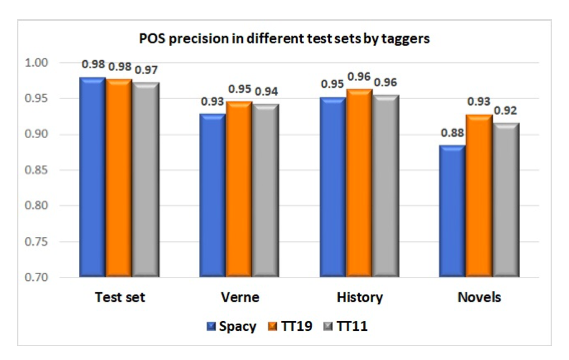
\includegraphics[width=.7\textwidth]{images/pos_tagger.png}
\caption{Preciznost alata za određivanje vrsta reči na različitim skupovima podataka}
\label{img:pos_tagger}
\end{figure}

\section{Lematizacija}

Proces lematizacije jeste onaj u kome se za svaku reč nalazi njena kanonska forma, tačnije lema. U srpskom jeziku, za imenice lema je nominativ jednine,  za glagole infinitiv, a za prideve nominativ jednine muškog roda. 

Postoje dve metode za rešavanje problema lematizacije.  Prvi, da se prema obliku reči otklanja sufiks i nalazi njena lema. Ovaj oblik rešavanja ne daje tako dobre rezultate.  Drugi pristup uključuje korišćenje skupa podataka koji za svaku reč, za svaku njenu moguću vrstu reči, ima određenu lemu. Postoji mogućnost i kombinovanja ova dva pristupa. 
\newpage
\noindent
Algoritam korišćen u ovom radu za dobijanje vrsta reči je korišćen i za dobijanje lema. Korišćen je srpski morfološki rečnik koji sadrži sve dozvoljene parove vrsta reči i lema za određenu reč.

Ovaj algoritam nije pravi lematizator, već na najverovatniju vrstu reči za određenu reč pridruži lemu koja se nalazi u rečniku. Zbog ovakvog pristupa, reči koje za istu vrstu reči imaju različite leme ne mogu da postoje u rečniku \cite{tagger}.

Na slici \ref{img:lemmatization} je prikazana preciznost tri različita modela lematizatora trenirana na različitim skupovima podataka. Slika je preuzeta iz \cite{tagger}.

\begin{figure}[h!]
\centering
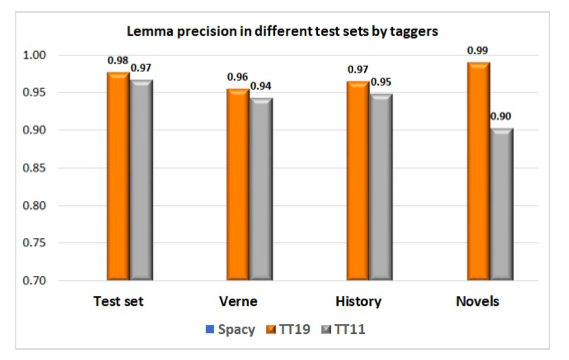
\includegraphics[width=.7\textwidth]{images/lemmatization.png}
\caption{Preciznost lematizatora na različitim skupovima podataka}
\label{img:lemmatization}
\end{figure}

\section{Skup podataka pre i nakon obrade}

Skup podataka koji će biti korišćen za eksperimente u ovom radu sadrži sakupljene podatke na već opisan način, koji su zatim obrađeni pomenutim tehnikama. Intervjua sa pacijentima obolelim od demencije Alchajmerovog tipa ima 22, koje nazivamo "pozitivni" i nalaze se u fascikli "P". Intervjua sa starijim licima koji nemaju utvrđenu demenciju Alchajmerovog tipa ima 57 i oni se nalaze u fascikli "N", a nazivamo ih "negativni". Nakon procesa određivanja vrste reči i leme za svaku reč intervjua, za svaki transkript je kreiran novi dokument koji u sebi sadrži potrebne informacije. 
\newpage
\noindent
Ako se u transkriptu nalazi rečenica:
\newline
\newline
\noindent\fbox{
    \parbox{\textwidth}{
      Ja sam Bojana.  
    }
}
\newline
\newline
onda će se u odgovarajućoj datoteci naći i sledeći redovi, gde u svakom redu prva reč označava izvorni oblik reči, druga vrstu, a treća lemu.
\newline
\newline
\noindent\fbox{
    \parbox{\textwidth}{
      Ja	PRON	Ja\newline
	sam	AUX	jesam\newline
	Bojana	PROPN	Bojana\newline
	.	PUNCT	.
    }
}
\newline
\newline

\chapter{Problem klasifikacije}

Pojam mašinskog učenja se vezuje za programe koji na osnovu podataka "uče" kako da se ponašaju i zaključuju na prethodno nepoznatim podacima. Osnovna podela metoda mašinskog učenja je na nadgledano (eng. supervised), nenadgledano (eng. unsupervised) učenje i učenje potkrepljivanjem (eng. reinforcement learning) \cite{MladenAndjelka}. Karakteristika nadgledanog učenja je da se svaka instanca sastoji iz podatka od kog se uči i iz onoga što je potrebno naučiti. U slučaju klasifikacije, ono što se uči je sama klasa ili skup klasa koje se pridružuju podatku. Ova metoda rešava mnoge probleme, kao što je problem prepoznavanja lica, utvrđivanje prisustva bolesti i slično. Nenadgledano učenje se razlikuje po tome što instanca ne sadrži ono što je potrebno naučiti. Ove metode su fokusirane na nalaženje strukture u podacima, kao što je rešavanje problema klasterovanja. Učenje potkrepljivanjem se koristi tamo gde je neophodno preduzeti niz akcija na osnovu stanja okruženja. Primer za ovu vrstu metoda je problem autonomne vožnje \cite{MladenAndjelka}.

Problem klasifikacije je jednostavan, od N klasa treba odrediti ispravnu za svaku instancu. Ulazni skup podataka koji se klasifikuje se sastoji od instanci. Klasifikacija spada u nadgledano učenje, zato što su podaci koji se korste labelirani, uz sam podatak postoji i ranije određena klasa. Podaci se dele na dva skupa, za trening i test. Skup za trening služi da se nauče pravilnosti i izgradi model, a skup za test služi za evaluaciju klasifikatora. Svi podaci prolaze korak pretprocesiranja koji uključuje obradu podataka kako bi ovaj proces bio uspešniji. Kreira se klasifikator, tačnije klasifikacioni model koji za zadatak ima da da preslika skup atributa instance x u neku od predefinisanih klasa y. 
\newline\newline\newline
Ulaz predstavlja skup atributa (eng. features), dok je izlaz najčešće jedna promenljiva koju nazivamo ciljnom promenljivom (eng. target variable). Ulaz se označava sa x, a izlaz sa y i obe promenljive su u vektorskom obliku.

Vrste klasifikacija se mogu podeliti po broju klasa, po tome da li može instanci biti dodeljeno više klasa ili samo jedna kao i po tipu klasifikacije.

Po broju klasa, podela je sledeća:

\begin{enumerate}
\item Binarna (eng. binary): postoje dve klase između kojih se bira i često odgovara na pitanje da li je nešto deo nekog skupa ili ne. Primer je detekcija nepoželjnih poruka ili prisustvo neke bolesti kod ispitanika.
\item Višeklasna (eng. multi-class): postoji više od dve klase između kojih se bira. Primer je prepoznavanje lica, klasifikacija vrste biljaka i slično. 
\end{enumerate}

Po tome da li može biti dodeljena samo jedna klasa ili više, podela je sledeća:

\begin{enumerate}
\item Jednoznačna (eng. single-label) - Jednoj instanci može biti dodeljena tačno jedna klasa
\item Višeznačna (eng.  multi-label) - Jednoj instanci se može pridružiti nula ili više klasa. Primer je kada na slici treba da se detektuju objekti, pa se očekuje prisutnost više objekata.
\end{enumerate}

Po tipu klasifikacije, razlikujemo sledeće:

\begin{enumerate}
\item Čvrsta (eng. hard) - Donosi se odluka da li instanca pripada klasi ili ne. 
\item Meka (eng. soft) - Instanci se pridružuje vrednost između 0 i 1 i time se određuje pripadnost klasi \cite{JelenaPHD}.
\end{enumerate}

\begin{figure}[h!]
\centering
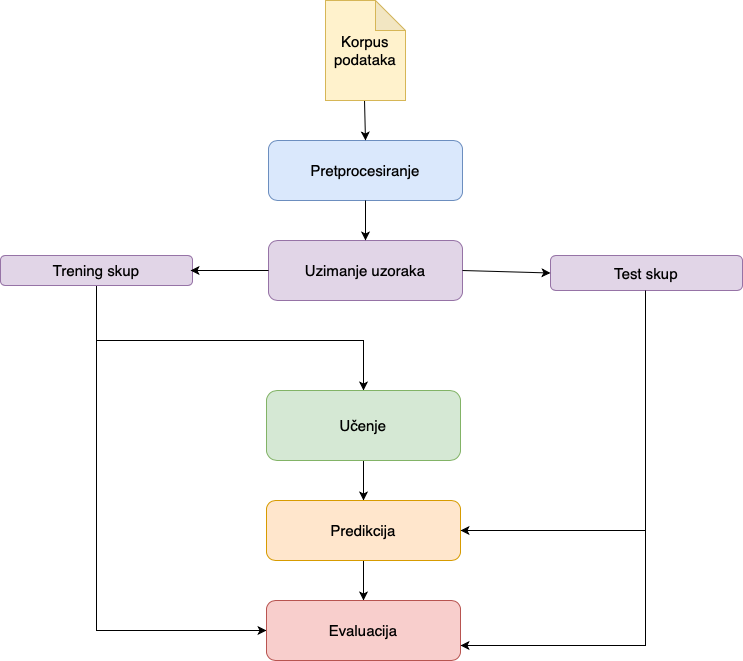
\includegraphics[width=.7\textwidth]{images/workflow.png}
\caption{Proces klasifikacije}
\label{img:workflow}
\end{figure}

Na slici \ref{img:workflow} je prikazan tok procesa klasifikacije. Prvi korak je skupljanje podataka i njihova obrada, zatim deljenje na test i trening skup. Na ovakvim skupovima se radi pretprocesiranje i obrada podataka. Trening skup zatim služi za treniranje klasifikatora. Uz pomoć tog istreniranog klasifikatora se radi predikcija na skupu za testiranje. Nakon toga, sledi neophodan korak evaluacije modela u koji ulazi procena performansi. Bitno je naglasiti da se većina ovih koraka ne izvodi jednom i svi koraci od učenja do evaluacije se izvode veliki broj puta kako bi se dobila najbolja moguća tačnost. Klasifikator se mora prilagoditi podacima. To činimo kako samim izborom klasifikatora, tako i podešavanjem njegovih parametara. U narednim sekcijama će bliže biti objašnjeni ovi koraci.  

\section{Podela korpusa}

Ulazni skup, korpus, se deli na dve grupe, za treniranje i za testiranje. Skup za treniranje se naziva trening skup i služi za kreiranje klasifikatora. Skup za testiranje se naziva testni skup i služi za evaluaciju klasifikatora. U većini slučajeva testni skup predstavlja manji deo korpusa od trening skupa.  Neophodno je da skupovi budu ravnopravno raspodeljeni, što znači da u svakom skupu treba da se nađe određeni procenat svih klasa koje razmatramo. Tehnike koje pokusavaju da zadovolje zahtev da podskupovi (trening i test skup) imaju istu raspodelu atributa i ciljne promenljive nazivaju se tehnikama stratifikacije.  Korpus delimo na ove dve grupe na osnovu jedne karakteristike koja je izabrana, a u slučaju klasifikacije je najčešće to baš ona karakteristika koja određuje kojoj klasi uzorak pripada. U slučaju klasifikacije obolelih od Alchajmerove bolesti karakteristika koju biramo je pripadnost pozitivnom i negativnom skupu, tačnije da li je osoba obolela od Alchajmerove bolesti ili ne. 

Uz treniranje i testiranje, dodatan korak je validacija, koji nije obavezan. Ovaj korak služi za procenu performansi, podešavanje parametara i biranje modela, kako bi bili dobijeni što bolji rezultati u koraku evaluacije. 
\newpage
U idealnom slučaju, korpus bi bio podeljen na test i trening deo, tako da se treniranje i validacija rade na trening, a evaluacija samo na test skupu. Uobičajeno je da se radi ugnježdena 10-struka unakrsna validacija (eng. cross validation).  
U ovoj metodi se korpus deli na 11 delova, gde se 10 delova uzima za trening i validaciju, a 1 deo za evaluaciju, što se može videti na slici \ref{img:corss1} koja je preuzeta iz \cite{cross}.  U procesu validacije se izvodi 10 iteracija, gde se trening vrši na 9, a testiranje i dodatno podešavanje parametara na jednom preostalom skupu. U svakoj iteraciji se taj skup za testiranje i podešavanje parametara menja.  Ovaj postupak je prikazan na slici \ref{img:corss2}, a ona je preuzeta iz \cite{cross}, gde $E_i$ predstavlja vrednost odabranog parametra u tekućoj iteraciji. Korak evaluacije se u ovom slučaju vrši na jednom skupu koji do tada nije korišćen, koji je na slici \ref{img:corss1} označen crveno. 
U slučaju podataka koji se koriste za eksperimente u ovom radu, skupovi pozitivnih i negativnih su podeljeni na po tri podskupa, pa se skup za treniranje sastoji iz dva podskupa pozitivnih i 2 podskupa negativnih, a skup za testiranje iz trećeg podskupa pozitivnih i trećeg podskupa negativnih.  U idealnom slučaju, testni skup ne učestvuje u procesu unakrsne validacije, ali u eksperimentima rađenim u ovom radu to nije bilo moguće, zbog malog broja instanci koje su prikupljene.  U ovom slučaju će unakrsna validacija biti rađena na sva tri skupa.

\begin{figure}[h!]
\centering
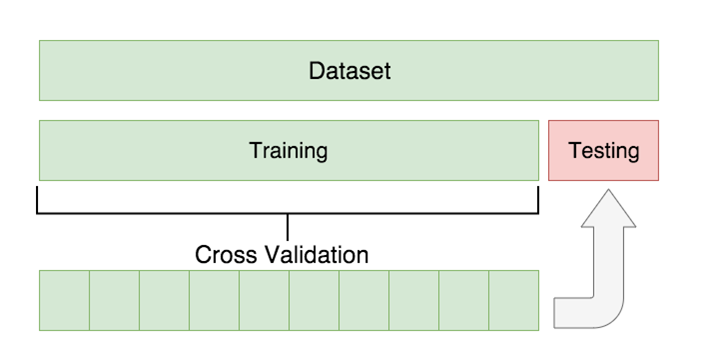
\includegraphics[width=.7\textwidth]{images/corss1.png}
\caption{ugnježdena 10-struka unakrsna validacija / podela korpusa podataka}
\label{img:corss1}
\end{figure}

\begin{figure}[h!]
\centering
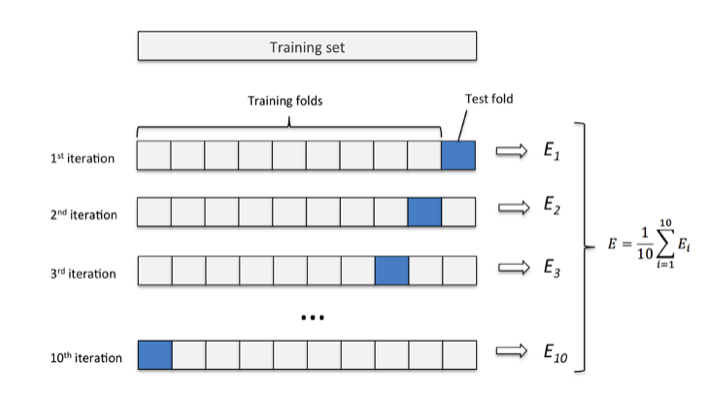
\includegraphics[width=.7\textwidth]{images/corss2.png}
\caption{ugnježdena 10-struka unakrsna validacija / podela korpusa podataka, gde $E_i$ predstavlja vrednost odabranog parametra u tekućoj iteraciji}
\label{img:corss2}
\end{figure}

\section{Pretprocesiranje}
 
Pretprocesiranje je korak koji nije obavezan, ali može značajno poboljšati performanse klasifikatora. Pretprocesiranje se koristi za prečišćavanje teksta, uklanjanje reči koje nisu bitne za klasifikaciju i za uniformisanje reči. 
\newpage
Metode pretprocesiranja teksta su različite, u zavisnosti od podataka koji se koriste. Nakon prikupljanja podataka, korpus predstavljaju sirovi podaci. Svaki tekst se deli na reči i zatim se pristupa nekim od tehnika pretprocesiranja:
\begin{enumerate}
\item Određivanje vrsta reči
\item Stemovanje
\item Lematizacija
\item Uklanjanje razmaka
\item Uklanjanje stop reči
\item Uklanjanje znakova interpunkcije
\item Prevođenje velikih slova u mala
\item Normalizacija teksta
\end{enumerate}

\textbf{Određivanje vrsta reči} je postupak gde se svakoj reči u rečenici pridružuje njena vrsta. U prethodnom poglavlju je bliže objašnjen algoritam po kome funkcioniše korišćeni program.

\textbf{Stemovanje} je proces uklanjanja sufiksa ili prefiksa reči. Ovim postupkom se nalazi koren reči. Problemi koji se mogu susresti su prekomerno ili premalo stemovanje, kada se uklanja veći ili manji deo reči nego što treba.

\textbf{Lematizacija} je sličan proces procesu stemovanja, sa tom razlikom da se reč preslikava u njen oblik iz rečnika, tačnije lemu. U okviru prethodnog poglavlja je detaljnije objašnjen proces lematizacije kao i algoritam korišćen u ovom radu. Stemovanjem i lematizacijom se reči koje su zapisane u različitim oblicima, a imaju isto značenje, prevode u isti oblik.

\textbf{Uklanjanje razmaka i znakova interpunkcije} je jednostavan zadatak, a bitno je ukloniti ih pošto nemaju značaj u razumevanju teksta.
 
\textbf{Prevođenje velikih slova u mala} je takođe sa strane implementacije jednostavan zadatak, a često se previdi. Ovaj korak pomaže u tome da se unifikuju reči i da nije bitno gde u rečenici je izgovorena reč i da li je napravljena greška u kucanju.

Korak \textbf{uklanjanja stop reči} se sastoji iz uklanjanja reči koje se često pojavljuju u jeziku. Neke od stop reči koje su korišćene u ovom istraživanju su "bi", "da", "li", "čega", "će", "ću", "ga", "ja" i slične. Stop reči nisu relevantne za klasifikaciju, pa se uklanjaju da ne bi skidale fokus sa onih koje su bitne.

Korak \textbf{normalizacije} teksta se izvodi tako što se svaka reč koja se nalazi u nestandardnom obliku prevodi u kanonski oblik. Ovaj korak je bitan ukoliko se u tekstu nalaze žargonski izrazi, skraćenice i slično.

U okviru ovog rada su koraci određivanja vrsta reči i lematizacija odrađeni pre deljenja teksta na skupove za testiranje i treniranje. U okviru metoda mašinskog učenja koje će biti prikazane u nastavku su korišćeni koraci uklanjanja razmaka, stop reči i razmaka, kao i prevođenje velikih slova u mala.

\section{Vektorska reprezentacija teksta} \label{sec:vrt}

Korpus podataka se sastoji od tekstova podeljenih u klase kojima pripadaju. Tekst u svojoj klasičnoj formi nije pogodan ulaz za algoritme mašinskog učenja.  Pošto se na ulazu očekuju numeričke vrednosti,  potreban je mehanizam koji će preslikati tekst u brojčani format na neki logičan način.  Taj korak se naziva ugrađivanje reči (eng.  word embedding) \cite{wordembedding}.  Atribut teksta je osnovna jedinica teksta koja je izabrana da njome bude predstavljen tekst i za to postoji više mogućnosti. 
\newpage
Neke od njih su:
\begin{enumerate}
\item Vreća reči
\item N-grami reči
\item N-grami karaktera
\item N-grami bajtova
\end{enumerate}
Atributu se zatim dodeljuju težine.  Svaki od ovih načina dodeljivanja težina može biti primenjen na sve vrste atributa teksta. Neki od njih su:
\begin{enumerate}
\item 0 i 1
\item Frekvencija
\item FA-IFD metrika
\end{enumerate}

U narednim sekcijama biće prikazani atributi teksta kao i načini dodeljivanja težina atributima.

\subsection{Vreća reči}
Vreća reči (eng. bag-of-words) je jednostavna tehnika reprezentacije teksta. Ovom reprezentacijom se prikazuje koliko puta se neka reč nalazi u dokumentu.  Redosled reči u rečenici nije bitan,  pa je odatle i dobila svoje ime ”vreća”.  Ova reprezentacija takođe omogućava da ulaz u algoritam mašinskog učenja bude vektor fiksne dužine. Vreća reči, i pored toga što se kontekst i semantika zanemaruju,  često daje dobre rezultate.  
Pretprocesiranje dokumenata pre prevođenja u ovu reprezentaciju je bitno zato što su skupovi nad kojima se uči tipično jako veliki, a ovaj korak će smanjiti dimenziju rečnika koji se kreira.
U okviru programskog jezika \textit{Python} postoji biblioteka \textit{Sklearn} koja u sebi sadrži \textit{CountVectorizer} objekat koji je korišćen za eksperimente u ovom radu. 
Na primeru će biti pokazano kako se kreira vreća reči:

\begin{enumerate}
\item Predstavljanje skupa podataka
\newline
Pretpostavimo da nam skup podataka u ovom primeru predstavljaju sledeća 3 dokumenta:
\newline
\newline
\noindent\fbox{
    \parbox{\textwidth}{
    	1. Zorica voli da vežba u teretani. \newline
	2. Jovana voli da vežba jogu uveče.\newline
	3. Marko ne voli da vežba, ali voli da šeta u šumi.
    }
}
\newline
\newline
\item Pretprocesiranje i deljenje na reči
\newline
Kao korak pretprocesiranja,  uklonjeni će biti svi znakovi interpunkcije,  svi nepotrebni razmaci i sva slova će biti prevedena u mala,  uklonjene su stop reči i izvršena je lematizacija. U sledećem koraku će svaki dokument biti podeljen na reči.  Dokumenti sada izgledaju ovako:
\newline
\newline
\noindent\fbox{
    \parbox{\textwidth}{
    	1. "zorica", "voleti", "vežbati", "teretana" \newline
	2. "jovana", "voleti", "vežbati","joga",  "uveče"\newline
	3. "marko", "ne", "voleti", "vežbati", "voleti", "šetati", "šuma"
    }
}
\newline
\newline
\item Rečnik
\newline
Zatim kreiramo rečnik od svih reči koje se nalaze u svim dokumentima korpusa koji su prikazani u prošlom koraku.  Reči su sortirane. 
\newline
\newline
\noindent\fbox{
    \parbox{\textwidth}{
    	["joga", "jovana",  "marko", "ne", "šetati", "šuma", "uveče", "vežbati", "voleti", "teretana", "zorica" ]
    }
}
\newline
\newline
\item Predstavljanje dokumenata vrećom reči
\newline
U sledećem koraku transformišemo dokumente na osnovu pojavljivanja reči iz rečnika. 
\newline
\newline
\noindent\fbox{
    \parbox{\textwidth}{
    	1.  [0, 0, 0, 0, 0, 0, 0, 1, 1, 1, 1] \newline
	2.  [1, 1, 0, 0, 0, 0, 1, 1, 1, 0, 0] \newline
	3. [0, 0, 1, 1, 1, 1, 0, 1, 2, 0, 0]
    }
}
\newline
\newline
Trening skup se iz početnog koji sadrži dokumente transformiše u niz od n elemenata, gde je n broj dokumenata u korpusu.  Svaki element je jedan niz koji ima m elemenata, gde je m dužina rečnika.  Testni skup se na identičan način preslikava iz dokumenata u niz vektora.  
Vrećom reči je reprezentovan samo broj pojavljivanja reči u dokumentu.  
\newpage
\noindent
Ako se neka reč pojavljuje mnogo puta, to ne mora nužno značiti da je ona bitna.  Možda se samo često pojavljuje u tom skupu podataka ili je reč koja se često izgovara.
\end{enumerate}

\subsection{N-grami}

\newtheorem{mydef}{Definicija}
\begin{mydef}
Za datu sekvencu tokena S = \normalfont($s_1$,$s_2$,...,$s_{N+(n-1)}$\normalfont) , gde su N i n pozitivne celobrojne vrednosti,  n-gram sekvence S je podsekvenca uzastopnih tokena dužine n.  i-ti n-gram sekvence S je sekvenca ($s_i$, $s_{i+1}$, ..., $s_{i+n-1}$) \cite{ngram}.
\end{mydef}

N-gram predstavlja n sekvencijalnih elemenata.  N-grami se mogu definisati na nivou reči, karaktera i bajta.  N-grami na nivou karaktera i bajta su kod jezika koji se pišu latiničnom azbukom slični, zato što je jedan karakter predstavljen jednim bajtom, ali to nije slučaj kada su u pitanju na primer azijski jezici.  N-gramski model pokušava da nauči šablon sekvenci.  Ovom modelu su bitne i relacije između elemenata, odnosno, koji element se pojavljuje blizu kog.  N-gramski model donekle čuva poredak reči, a razmatra se verovatnoća da se određeni element \textit{e} nađe posle određene sekvence elemenata \textit{s}. 
Korišćenje n-grama se u okviru procesa obrade prirodnih jezika pokazalo kao efikasno.  Ova tehnika se koristi često u predviđanju reči koje se nadovezuju na datu rečenicu, ispravljanju grešaka u pisanju, generisanju teksta i slično.  
N-grami su relativno neosetljivi na pravopisne greške i jednostavni za implementaciju, pa se pre korišćenja ovog modela ne radi korak pretprocesiranja teksta, već samo izbacivanje znakova interpunkcije.  
Kod n-gramskih modela se \textit{n} bira prema prirodi problema i podataka,  ali se najčešće koriste brojevi do n=5.  Kada je n=1 to su unigrami, kada je n=2 to su bigrami,  a kada je n=3 to su trigrami i tako dalje.  Nekada se koriste i njihove kombinacije. 
U nastavku će biti pokazani primeri n-grama reči.

\begin{enumerate}
\item Predstavljanje skupa podataka
\newline
Skup podataka u ovom primeru nam predstavljaju sledeća 3 dokumenta:
\newline
\newline
\noindent\fbox{
    \parbox{\textwidth}{
    	1. Zorica voli da vežba u teretani. \newline
	2. Jovana voli da vežba jogu uveče.\newline
	3. Marko ne voli da vežba, ali voli da šeta u šumi.
    }
}
\newline
\newline
\item Unigrami
\newline
Unigrami su n-grami gde je n=1. Ovaj model liči na vreću reči, sa razlikom da se kod n-grama ne vrši pretprocesiranje,  pa će biti više izdvojenih reči.  Kod unigrama nema oslanjanja na prethodnu sekvencu \textit{s}. 
Unigrami u primeru su sledeći:
\newline
\newline
\noindent\fbox{
    \parbox{\textwidth}{
    	1. "zorica", "voli", "da",  "vežba", "u", "teretani" \newline
	2. "jovana", "voli", "da", "vežba", "jogu",  "uveče"\newline
	3. "marko", "ne", "voli", "da", "vežba","ali", "voli", "da", "šeta", "u", "šumi"
    }
}
\newline
\newline
\item Bigrami
\newline
Bigrami su n-grami gde je n=2.  Sekvenca elemenata \textit{s} koja se nalazi pre elementa koji se trenutno gleda je samo jedna reč.  Bigrami su u stanju da uzmu u obzir i negaciju, zato što gledaju dve reči zajedno, pa ovakvi modeli mogu dati i bolje rezultate \cite{ngram}.
   
Bigrami u primeru su sledeći: 
\newline
\newline
\noindent\fbox{
    \parbox{\textwidth}{
    	1.  ("zorica", "voli"),("voli","da"), ("da", "vežba"), ("vežba", "u"), ("u", "teretani")  \newline
	2.  ("jovana", "voli"),  ("voli","da" ), ("da", "vežba"), ("vežba", "jogu"), ("jogu","uveče" ) \newline
	3.  ("marko", "ne"), ("ne", "voli"), ("voli", "da"), ("da", "vežba"), ("vežba", "ali" ), ("ali", "voli" ),("voli","da" ), ("da", "šeta"), ("šeta", "u"), 		("u","šumi")
    }
}
\newline
\newline
\item Trigrami
\newline
Trigrami su n-grami gde je n=3. Trigrami u primeru su sledeći:
\newline
\newline
\noindent\fbox{
    \parbox{\textwidth}{
    	1.  ("zorica","voli", "da"),("voli","da", "vežba"), ("da", "vežba", "u"), ("vežba","u","teretani")\newline
	2.  ("jovana", "voli", "da"),  ("voli","da","vežba" ), ("da", "vežba", "jogu"), ("vežba", "jogu", "uveče") \newline
	3.  ("marko", "ne", "voli"), ("ne", "voli", "da"), ("voli", "da", "vežba"), ("da", "vežba", "ali"), ("vežba","ali", "voli"), ("ali", "voli","da"),			("voli","da","šeta"), ("da", "šeta","u"), ("šeta", "u", "šumi")
    }
}
\newline
\newline
\end{enumerate}
\noindent
Na prethodnom primeru je prikazan način na koji se grade n-grami reči. Na isti način se grade i n-grami karaktera i bajtova.  
\subsection{Frekvencija atributa - FA}

\textbf{Frekvencija atributa (eng. term frequency)} se označava sa FA (eng. TF) i meri učestalost pojavljivanja reči u dokumentima.  Učestalije reči imaju veću važnost od onih manje učestalih.  FA mera pokazuje koliko se često određeni atribut \textit{w} nalazi u dokumentu. Da bi se izbegao slučaj da neka reč koja ima veću frekvenciju pojavljivanja, ima i veću bitnost, samim tim što je dokument veći, uvodi se normalizacija tako što se broj pojavljivanja reči u tekstu podeli sa ukupnim brojem reči u tekstu.  Ovaj model daje bolje rezultate ukoliko je u okviru pretprocesiranja odrađeno izbacivanje stop reči, kao i uklanjanje znakova interpunkcije i lematizacija.  Frekvencija atributa se može kreirati nad vrećom reči kao i nad n-gramima.

Računa se po formuli za reč \textit{w} i dokument \textit{d}:

\begin{equation}
	FA(w,d) = \frac{\text{broj pojavljivanja reči w u dokumentu d}}{\text{broj svih reči u dokumentu d}}
\end{equation}

\subsection{Inverzna frekvencija dokumenta - IFD}

\textbf{Frekvencija dokumenta (eng.  document frequency)} označava se kao FD (eng.  DF) i  definiše kao broj dokumenata u kojima se pojavljuje atrubut \textit{w}.  Uvodimo oznaku:
\begin{equation}
	FD(w) = \text{broj svih dokumenata u kojima se pojavljuje reč w}
\end{equation}

\textbf{Inverzna funkcija frekvencije dokumenta (eng.  inverse document frequency)} tog atributa se predstavlja kao broj dokumenata u korpusu u onosu na broj dokumenata u kojima se pojavljuje atribut \textit{w} i računa se po formuli:

\begin{equation}
	IFD(w) = \frac{\text{broj svih dokumenata u korpusu}}{\text{broj svih dokumenata u kojima se pojavljuje reč w}}
\end{equation}
\newline
Kada je korpus veliki,  vrednost inverzne frekvencije dokumenata može biti ogroman broj, pa se dodaje logaritamska funkcija.  Da bi se izbeglo deljenje sa nulom, ako se reč ne pojavljuje u dokumentu,  dodaje se vrednost 1, pa formula izgleda ovako:

\begin{equation}
	IFD(w) = log\left(\frac{\text{broj svih dokumenata u korpusu}}{FD(w) + 1}\right)
\end{equation}

\subsection{FA-IFD metrika}

Prethodne mere se mogu kombinovati u jednu koju nazivamo \textbf{FA-IFD (eng.  TD-IDF)}, kojom se pronalaze atributi koji imaju veliku frekvenciju atributa,  a malu frekvenciju dokumenata, zato što je cilj da se da na važnosti atributima koji su frekventni u pojedinačnim, a da se retko pojavljuju u ostalim dokumentima \cite{JelenaPHD}.  Ova mera je zapravo proizvod prethodnih mera i formula izgleda ovako:

\begin{equation}
	FA-IFD(w, d) = FA(w,d) * IFD(w)
\end{equation}

FA-IFD mera se može kreirati nad vrećom reči kao i nad n-gramima.  U implementaciji ovog rada će biti prikazane obe opcije.

\section{Kreiranje i treniranje modela}

Za treniranje modela neophodno je odrediti algoritam koji će se koristiti za kreiranje klasifikatora. U zavisnosti od prirode problema, vrste i količine podataka, bira se algoritam koji će dati najbolje performanse. Klasifikator se trenira samo nad podacima za trening, što je prikazano na slici \ref{img:workflow}. U ovom koraku se na podacima koji su raspoloživi u skupu za treniranje model "uči" i nalazi pravilnosti, pa kreira model. U narednom koraku na osnovu prethodno kreiranog modela se vrši korak predikcije, a koriste se podaci iz testnog skupa, koji nije korišćen u koraku treniranja. U ovom koraku se predviđa klasa za svaku instancu skupa. 

\section{Evaluacija modela}

Poslednji korak je određivanje koliko je model koji je napravljen zapravo dobro istreniran. Poređenjem predviđene klase i one stvarne dolazimo do zaključaka. Jedan od problema koji se može javiti je problem previše prilagođenog modela, a javlja se ukoliko se klasifikator previše prilagodi podacima za treniranje. Ovaj problem se može detektovati tako što su rezultati na skupu za treniranje dobri, dok su performanse na test skupu loše.  Najčešće se javlja kada se šum u ulaznim podacima predstavi kao bitan element \cite{JelenaPHD}.

Instance koje se nalaze u test skupu nisu korišćene za kreiranje modela i za svaku od njih klasifikator predviđa klasu. Nakon ovog koraka se uz svaki dokument iz test skupa nalaze dve klase, ona koju znamo da je tačna i ona dodeljena klasifikatorom. Svaki dokument može biti ispravno i neispravno klasifikovan i prema tome može biti u skupu:

\begin{enumerate}
\item Stvarno pozitivni SP (eng. True Positives, TP)
\item Lažno pozitivni LP (eng. False Positives, FP)
\item Stvarno negativni SN (eng. True Negative, TP)
\item Lažno negativni LN (eng. False Negative, FN)
\end{enumerate}
\noindent
gde je stvarno pozitivni broj instanci koje su zaista pozitivne i koje je klasifikator označio kao pozitivne. Lažno pozitivni je broj instanci koje su negativne, a koje je klasifikator označio kao pozitivne. Stvarno negativni je broj instanci koje su negativne, a koje je klasifikator označio kao negativne. Lažno negativni je broj instanci koje su pozitivne, a koje je klasifikator označio kao negativne. Njihov zbir treba da bude jednak broju instanci u testnom skupu.

Ova četiri podatka definišu matricu konfuzije (eng. confusion matrix). Matrica konfuzije je NxN matrica koja se koristi za evaluaciju klasifikacionog modela, gde je N broj klasifikacionih klasa. U slučaju višeklasne klasifikacije element matrice C\textsubscript{ij} predstavlja broj elemenata koji pripadaju klasi i, a klasifikovani su u klasu j \cite{JelenaPHD}. Model je bolji što je više elemenata van dijagonale u matrici jednako nula. Matrica konfuzije za binarnu klasifikaciju je prikazana na slici \ref{img:confusionMatrix}.

\begin{figure}[h!]
\centering
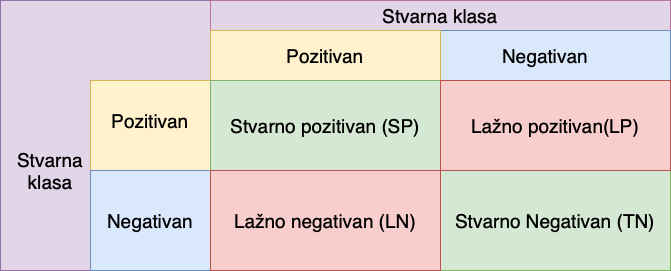
\includegraphics[width=.7\textwidth]{images/confusionMatrix.png}
\caption{Matrica konfuzije}
\label{img:confusionMatrix}
\end{figure}
\newpage
Ove podatke koristimo za procenu koliko je model dobro istreniran pomoću određenih mera, a neke od njih su sledeće:

\begin{enumerate}
\item Tačnost klasifikacije
\item Preciznost klasifikacije
\item Odziv klasifikacije
\item F-mera
\end{enumerate}

\textbf{Tačnost klasifikacije (eng. accuracy)} prikazuje odnos tačno klasifikovanih instanci i svih klasifikovanih instanci i računa se po formuli:

\begin{equation}
	acc = \frac{SP+SN}{SP+SN+LP+LN}
\end{equation}
\noindent
Vrednosti tačnosti klasifikacije se kreću između 0 i 1.

\textbf{Preciznost klasifikacije (eng. precision)} prikazuje odnos pozitivnih instanci koje su tako klasifikovane i svih instanci koje su klasifikovane pozitivno i računa se po formuli:

\begin{equation}
	P = \frac{SP}{SP+LP}
\end{equation}
\noindent
Ova mera pokazuje koliko je instanci pogrešno klasifikovano kao pozitivno. Ako model nema lažnih pozitiva (LP), onda će vrednost preciznosti biti 1, tačnije 100\%. Što više lažnih pozitiva ima, to će preciznost biti lošija. Vrednosti preciznosti se kreću između 0 i 1.

\textbf{Odziv klasifikacije (eng. recall)} je mera koja prikazuje odnos pozitivnih instanci koje su tako klasifikovane i zbira pozitivnih instanci koje su tako klasifikovane i pozitivnih instanci koje su klasifikovane kao negativne. Ova mera se fokusira na broj pozitivnih instanci koje su pogrešno klasifikovane(lažno negativne) . Ako su sve pozitivne instance upravo tako klasifikovane, onda će vrednost odziva biti 1, tačnije 100\%.  Vrednosti odziva se kreću između 0 i 1.Računa se po formuli:

\begin{equation}
	R = \frac{SP}{SP+LN}
\end{equation}
\noindent
Preciznost je bitna mera kada nam je bitnija mera lažno pozitivnih od lažno negativnih. Preciznost je bitna mera u sistemima gde je bitno da se ne dobije negativan rezultat, dok je odziv bitna mera u sistemina gde je problem ako pozitivan slučaj prođe nezapaženo.

\textbf{F-mera} predstavlja harmonijsku sredinu preciznosti i odziva,  a razmatra i lažno pozitivne i lažno negativne. Računa se po sledećoj formuli:

\begin{equation}
	F = \frac{2}{\frac{1}{P} + \frac{1}{R}} = \frac{2 * P * R }{P + R}
\end{equation}

\noindent
Vrednosti f-mere se kreću između 0 i 1.


U slučaju implementacije prikazane u ovom radu,  biće vršen proces unakrsne validacije, ali ne samo na trening skupu, već na celom korpusu.  Ovaj proces je prikazan na slici \ref{img:K_cross_validation},  gde svaki red predstavlja jednu iteraciju treniranja, testiranja i evaluacije, ljubičasti kvadrat prikazuje skup za testiranje, a beli kvadrati skupove za treniranje.  U idealnom slučaju, skup za testiranje bi bio na početku izdvojen i na njemu ne bi bio vršen korak unakrsne validacije, već samo evaluacija, ali na ovom skupu to nije moguće zbog količine podataka koju sadrži. 


\begin{figure}[h!]
\centering
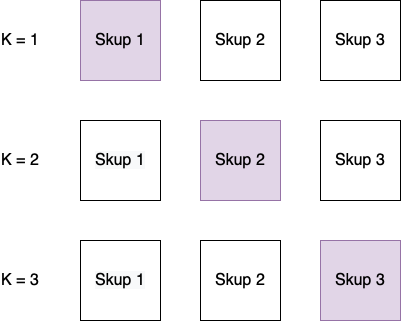
\includegraphics[width=.7\textwidth]{images/K_cross_validation.png}
\caption{Unakrsna validacija}
\label{img:K_cross_validation}
\end{figure}


\chapter{Rešavanje problema metodama lingvističke analize}
\label{poglavlja:ling}

Lingvistička analiza teksta, u ovom kontekstu, predstavlja pokušaj da se korišćenjem računara donose neki zaključci na osnovu reči u tekstu, njihovih vrsta u rečenicama, frekvenciji pojavljivanja i slično. Da bi računar "razumeo" pisani tekst, prvo je neophodno podeliti ga na rečenice. Mnogi lingvistički alati se baziraju na analizi jedne po jedne rečenice. Zatim se izvodi proces tokenizacije, deljenja rečenice na pojedinačne reči. Nakon toga se izvodi korak lematizacije, prevođenja svake reči u njen osnovni oblik, tačnije lemu. U nekim slučajevima, ovaj korak obuhvata i čišćenje, tačnije ispravljanje pogrešno napisanih reči. Poslednji korak je dodeljivanje vrsta reči svakoj od njih.

Pacijenti oboleli od Alchajmerove bolesti kao jedan od simptoma imaju gubitak sposobnosti funkcionalne komunikacije i probleme u lingvističkim veštinama. Procenjivanje afazije kod pacijenata obolelih od demencije Alchajmerovog tipa je vrlo zahtevan zadatak. Koristeći različite metrike nad vrstama reči koje su dobijene iz spontanog govora obolelih, pokušavamo da pronađemo pravilnost i da tako dođemo do zaključaka i mogućnosti klasifikacije na obolele i zdrave pojedince.

U mnogim naučnim radovima koji se bave temom Alchajmerove bolesti predstavljaju se upravo lingvističke mere kao način razlikovanja obolelih od zdravih pojedinaca i metod za uočavanje pravilnosti u njihovom govoru. Potrebno je naći pravilnost u načinu na koji pojedinac govori i koristi svoj vokabular, koliko često izgovara neke vrste reči, koliko su dugačke rečenice. Neki od primera korišćenja ovih mera se mogu naći u radovima, \cite{automaticdetandrat}, \cite{Evaloftechfolexicalperformance} i \cite{linguisticfeatures}.

\section{Lingvističke mere}

Korišćeno je ukupno šesnaest lingvističkih mera u okviru ovog rada. Mere bazirane na vrstama reči uključuju frekvenciju pojavljivanja određene vrste reči u tekstu, kao i tu vrednost normalizovanu ukupnim brojem reči u tekstu. Takođe, koriste se tri mere koje govore o bogatstvu vokabulara: Odnos tipa tokena (eng. Type Token Ratio), Bruneov index (eng. Brunet's Index) i Onoreova statistika (eng. Honore's Statistic)koje počivaju na bogatstvu vokabulara\cite{automaticdetandrat}.

Za svaki tekst se izračunava dužina teksta (N) kao broj izgovorenih reči i prosečna dužina izgovorenih reči. Vokabular (V) je mera koja pokazuje koliko različitih reči se pojavljuje u tekstu koji se obrađuje. Vokabular reči izgovorenih jednom (V\textsubscript{1}) se izračunava tako što se od reči koje se nalaze u vokabularu broje samo one koje su izgovorene jednom. Ove mere se koriste kako samostalno, tako i za izračunavanje mera koje počivaju na bogatstvu vokabulara.

\section{Mere bazirane na vrstama reči}

Mera pojavljivanja pojedinačne vrste reči u tekstu se izračunava tako što se broji svako pojavljivanje te vrste reči. Pored toga, izračunavamo i frekvencije pojavljivanja različitih vrsta reči normalizovane ukupnim brojem reči u tekstu. U okviru ovog rada, razmatrane su mere vezane za broj imenica, glagola, prideva, priloga i zamenica kao i njihove normalizovane vrednosti. Od koristi mogu biti i odnosi između ovih vrednosti, pa se tako izračunavaju i odnos između broja pojavljivanja imenica i glagola, i zamenica i imenica kao i zamenica i glagola. Ove mere su izabrane heuristički i predstavljaju leksičku raspodeljenost izgovorenih reči.

Broj imenica pokazuje sposobnost ispitanika da koristi imenice i ona bi mogla biti osetljiva na probleme sa pronalaženjem reči od čega pate osobe koje imaju Alchajmerovu bolest. Broj zamenica je u kontrastu sa brojem imenica i koristi se kao merilo indirektnog referenciranja. Broj prideva prikazuje kvalitet govora obolele osobe, tačnije mogućnost za opisivanjem. Broj glagola se često koristi kao lingvistička mera i meri tečnost govora \cite{Evaloftechfolexicalperformance}. 

\section{Mere bazirane na bogatstvu vokabulara}
 
Tri mere koje se zasnivaju na bogatstvu vokabulara su: Odnos tipa tokena, Bruneov indeks i Onoreova statistika. Za njihovo izračunavanje neophodno je prvo izračunati dužinu teksta, bogatstvo vokabulara i bogatstvo vokabulara za reči izrečene jednom. Dužina teksta se meri kao broj reči koje se pojavljuju u tekstu i označava se sa N. Mera bogatstva vokabulara se izračunava tako što se broji koliko različitih reči se pojavljuje u tekstu i označava se sa V. Mera bogatstva vokabulara za reči izgovorene jednom se izračunava tako što se broje reči u tekstu koje se pojavljuju samo jednom. Ova mera se označava sa V\textsubscript{1}.

\subsection{Odnos tipa tokena}

Odnos tipa tokena se računa po formuli:

\begin{equation}
	TTR = \frac{V}{N}
\end{equation}

{\setlength{\parindent}{0cm}
gde je N dužina teksta, a V mera bogatstva vokabulara i predstavlja odnos ove dve vrednosti. Ova mera je osetljiva na dužinu teksta. Veće vrednosti Odnosa tipa tokena se povezuju sa bogatijim vokabularom.
}

\subsection{Bruneov Indeks}

Bruneov indeks se računa po formuli:

\begin{equation}
	W = N^{V^{-0,165}}
\end{equation}

{\setlength{\parindent}{0cm}
gde je N dužina teksta, a V mera bogatstva vokabulara. Ova mera se takođe povezuje sa bogatijim vokabularom, ali nije osetljiva na dužinu teksta.  Tipične vrednosti su između 10 i 20. Manje vrednosti se povezuju sa bogatijim govorom. 
}
\newpage
\subsection{Onoreova Statistika}

Onoreova Statistika se računa po formuli:

\begin{equation}
	R = \frac{100logN}{1 - \frac{V_1}{V}}
\end{equation}

{\setlength{\parindent}{0cm}
gde je N dužina teksta, a V mera bogatstva vokabulara, a V\textsubscript{1} bogatstvo vokabulara za reči izrečene jednom. Veće vrednosti se povezuju sa bogatijim govorom.
}

\section{Klasifikacija bazirana na lingvističkim merama}

Za izračunavanje mera pomenutih u prethodnim sekcijama, koje nazivamo lingvističkim, koriste se već obrađeni podaci u kojima je svakoj reči svakog teksta pridružena njena vrsta. Izračunavanje mera koristeći tako pripremljene tekstove nije teško. Mere izračunavamo za svaki tekst pojedinačno u korpusu koji sadrži kako pozitivno, tako i negativno klasifikovane tekstove. Mere čuvamo u okviru datoteke koja nosi ime ispitanika sa ekstenzijom \textit{txt}. Ovakve mere možemo koristiti za upoređivanje i vizuelno prikazivanje na grafikonima. Da bismo procenili koliko je neka od metrika korisna u proceni da li je neko oboleo od Alchajmerove bolesti ili ne, moramo na osnovu nje pokušati da klasifikujemo novi tekst kao pozitivan ili negativan. 

Korak treniranja modela u ovom slučaju je već odrađen, pošto već imamo sve metrike izračunate za trening skup. Vrednosti metrika iz trening skupa ćemo u koraku evaluacije porediti sa vrednostima metrika iz testnog skupa.

Korak evaluacije u ovom slučaju obuhvata procenu kvaliteta klasifikacije za svaku od metrika koje smo pomenuli u prethodnim sekcijama. Vrednosti metrike za jedan tekst iz testnog skupa poredimo sa svim vrednostima metrika iz trening skupa i prema blizini odlučujemo kom od skupova tekst iz testnog skupa treba da pripadne po našem klasifikatoru. Zatim se klasa poredi sa stvarnom klasom koju tekst nosi.
\newpage
\noindent
Ako pretpostavimo da trening i test skup sadrže sledeće dokumente:

\begin{equation}
	TRENING = {d\textsubscript{1}, d\textsubscript{2}, d\textsubscript{3},d \textsubscript{4}}
\end{equation}

\begin{equation}
	TEST = {d\textsubscript{5}}
\end{equation}

\noindent
gde dokumenti d\textsubscript{1}, i d\textsubscript{2} pripadaju skupu P, a dokumenti d\textsubscript{3}, i d\textsubscript{4} skupu N, a d\textsubscript{5} pripada skupu P i da radimo klasifikaciju po metrici X, onda sledi izračunavanje:

\begin{gather*}
	y\textsubscript{1} = \text{abs}(\text{X}(d\textsubscript{1}) - \text{X}(d\textsubscript{5})) \\
	y\textsubscript{2} = \text{abs}(\text{X}(d\textsubscript{2}) - \text{X}(d\textsubscript{5})) \\
	y\textsubscript{3} = \text{abs}(\text{X}(d\textsubscript{3}) - \text{X}(d\textsubscript{5})) \\
	y\textsubscript{4} = \text{abs}(\text{X}(d\textsubscript{4}) - \text{X}(d\textsubscript{5})) \\
	y\textsubscript{P} = y\textsubscript{1} + y\textsubscript{2} \\
	y\textsubscript{N} = y\textsubscript{3} + y\textsubscript{4}
\end{gather*}
\noindent
gde \text{X}(d\textsubscript{i}) predstavlja vrednost metrike X u dokumentu d\textsubscript{i}.

{\setlength{\parindent}{0cm}
Zatim se porede vrednosti y\textsubscript{P} i y\textsubscript{N}. Koja vrednost je manja, smatramo da dokument toj grupi pripada, pošto je ukupan zbir razlika vrednosti između dokumenta {d\textsubscript{5}} od dokumenta iz te grupe manji.

Sledeći korak je evaluacija modela koja je bliže opisana u sekciji 3.5. Nakon što su dobijene vrednosti, svaki dokument označavamo jednom od ovih oznaka:
}

\begin{enumerate}
\item Stvarno pozitivni SP (eng. True Positives, TP)
\item Lažno pozitivni LP (eng.  False Positives,  FP)
\item Stvarno negativni SN (eng.  True Negative, TP)
\item Lažno negativni LN (eng.  False Negative, FN)
\end{enumerate}


\chapter{Rešavanje problema metodom potpornih vektora}

Metoda potpornih vektora (eng. Support Vector Machine - SVM) je algoritam mašinskog učenja koji rešava problem klasifikacije. Ovaj klasifikator se bazira na vektorskim prostorima. Osnovni oblik algoritma je konsturisan za binarnu klasifikaciju. Ova metoda je jedna od najuspešnijih za klasifikaciju, a naročito dobre performanse pokazuje kada podaci imaju veliki broj atributa ili instanci u skupu. Ova metoda je prilično otporna na šum.

Ovaj algoritam se bazira na ideji da se podaci predstave u vektorskom prostoru, pa da se pronađe hiper-ravan takva da instance jedne klase budu sa jedne strane ravni, a instance druge klase sa druge. Takvih ravni je mnogo.

U fazi učenja se pronalazi optimalna hiper-ravan koja na najbolji mogući način razdvaja ove klase. Optimalna hiper-ravan je ona koja maksimizuje rastojanje do najbliže instance obe klase.Klasifikacioni model metoda potpornih vektora je zapravo jednačina te hiper-ravni. Razlog zbog kog se nalazi ravan koja ima najširi pojas praznog prostora oko sebe (tzv.  margine) jeste da bi se minimizovao rizik da se neka tačka pogrešno klasifikuje. Kada su podaci linearno razdvojivi, hiper-ravan koja predstavlja granicu je prava \cite{JelenaPHD}.

\begin{figure}[h!]
\centering
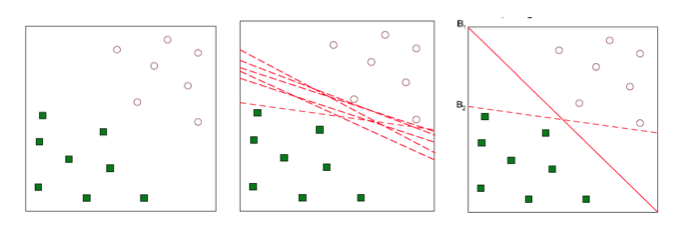
\includegraphics[width=.7\textwidth]{images/svm.png}
\caption{ Hiper-ravan u metodi potpornih vektora }
\label{img:svm_1}
\end{figure}

Na slici \ref{img:svm_1} prvo su prikazani podaci u dve klase. Jedna klasa je predstavljena belim kužićima, a druga klasa zelenim kvadratićima. U srednjem delu su prikazane neke od mogućih hiper-ravni koje razdvajaju ova dva skupa. Na desnom delu slike su predstavljene dve koje poredimo, $B_1$ i $B_2$. Slika je preuzeta iz knjige \cite{introductiontodm}. Kako je cilj da hiper-ravan maksimizuje veličinu margine od nje do najbližih instanci oba skupa, možemo zaključiti da treba izabrati $B_1$.

\begin{figure}[h!]
\centering
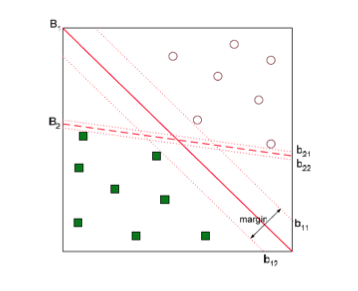
\includegraphics[width=.7\textwidth]{images/svm1.png}
\caption{ Hiper-ravan u metodi potpornih vektora sa marginom }
\label{img:svm_2}
\end{figure}

\noindent
Na slici \ref{img:svm_2} su grafički prikazane margine oko obe ravni i vidi se koja margina je veća. Slika je preuzeta iz knjige \cite{introductiontodm}.

Proces učenja kada se određuje optimalna hiper-ravan se radi, kao i u ostalim algoritmima klasifikacije, na skupu za treniranje. Kada se radi korak predikcije, za svaku instancu se određuje rastojanje od te ravni i prema tome sa koje strane se nalazi, dodeljuje joj se jedna od klasa.

Neka je dato \textit{n} objekata koje treba klasifikovati \textit{\normalfont($x_1$,$y_1$\normalfont),\normalfont($x_2$,$y_2$\normalfont),...,\normalfont($x_n$,$y_n$\normalfont)}, gde su $x_i \in R^n$ instance, a $y_i \in \{-1,1\}$ predstavlja klasu kojoj instanca pripada. Cilj je naći takvu hiper-ravan da razdvaja instance kojima je klasa $y$ = 1 i one kojima je $y$ = -1. Pretpostavimo da važi uslov linearne razdvojivosti. 
\newpage
\noindent
Jednačina hiper-ravni se predstavlja izrazom:
\begin{equation}
	w\cdot x+w\textsubscript{0} = 0
\end{equation}

{\setlength{\parindent}{0cm}
gde je \textit{w} vektor težina i određuje smer hiper-ravni, a $w_0$ pomeraj. Optimalna hiper-ravan je ona koja je maksimalno udaljena od najbližih predstavnika klasa. Te dve instance koje su najbliže predstavljaju potporne vektore i po njima je ova metoda i dobila ime. Jednačine dve ravni koje su paralelne sa optimalnom, a prolaze kroz te najbliže predstavnike klasa su:
}

\begin{equation}
	w\cdot x+w\textsubscript{0} = c \\
\end{equation}

\begin{equation}
	w\cdot x+w\textsubscript{0} = -c
\end{equation}

{\setlength{\parindent}{0cm}
Kada podelimo sve jednačine sa c, za neke nove parametre $w$ i $w_0$ dobijamo sledeće jednačine:
}

\begin{equation}
	w\cdot x+w\textsubscript{0} = 0
\end{equation}

\begin{equation}
	w\cdot x+w\textsubscript{0} = 1
\end{equation}

\begin{equation}
	w\cdot x+w\textsubscript{0} = -1
\end{equation}

\noindent
Jednačina rastojanja tačke x od hiper-ravni je sledeća:

\begin{equation}
	\frac{|w \cdot x + w\textsubscript{0}|}{\|w\|\textsubscript{2}}
\end{equation}

\noindent
pa tako dobijamo da je rastojanje između klasa u pravcu normalnom na optimalnu hiper-ravan sledeće:

\begin{equation}
	\frac{2}{\|w\|}
\end{equation}

\newpage
\noindent
Pošto pokušavamo da maksimizujemo ovo rastojanje, ako rešavamo optimizacioni problem minimizacijom, dobijamo sledeći izraz:

\begin{equation}
	\min_{w,w_0} \frac{\|w\|^{2}}{2} \\
\end{equation}

\begin{equation}
	y\textsubscript{i}(w \cdot x\textsubscript{i} + w_0) \geq 1 \text{ za i = } \overline{1,n}
\end{equation}

\noindent
Problem sa prethodnom logikom predstavlja činjenica da smo pretpostavili linearnu razdvojivost klasa. Na stvarnom skupu podataka, neophodno je prihvatiti neke greške i tada problem rešavamo metodom sa mekim pojasom ili pomoću kernela.

\subsection{Metod sa mekom marginom}

Za metod sa mekom marginom (eng. soft margin) uvodimo promenljive $\xi_i$ za $\overline{1,n}$ koje prikazuju koliko je instanca daleko od optimalne hiper-ravni ako je ona sa pogrešne strane.  Uvodi se i parametar C koji je nenegativan i kontroliše koliko težine se pridaje greškama. Ako je $C=0$, greške nisu važne, a ako je C veliko, onda su greške važne, a pravac hiper-ravni i širina pojasa nisu. Optimizacioni problem sada izgleda ovako:

\begin{equation}
	\min_{w,w_0} \frac{\|w\|^{2}}{2} + C \sum_{i=1}^{n} \xi_\textsubscript{i} \notag\\
\end{equation}

\begin{equation}
	y\textsubscript{i}(w \cdot x\textsubscript{i} + w_0) \geq 1 - \xi_\textsubscript{i} \text{ za i = } \overline{1,n} \notag\\
\end{equation}

\begin{equation}
	\xi_\textsubscript{i} \geq 0 \text{ za i = } \overline{1,n}
\end{equation}

\subsection{Kerneli (funkcije jezgra)}

Drugi način rešavanja problema u slučaju linearno nerazdvojivih podataka su kerneli. Kerneli su funkcije koje ulazni vektorski prostor preslikavaju u prostor veće dimenzije u kome je ulazni skup za učenje linearno razdvojiv. Oni transformišu linearno nerazdvojiv problem u linearno razdvojiv. U prostoru veće dimenzije je veća verovatnoća da se pronađe hiper-ravan koja razdvaja instance različitih klasa podataka \cite{JelenaPHD}.
\noindent
Koristi se preslikavanje:

\begin{equation}
	\Phi : x \rightarrow \varphi(x)
\end{equation}

\noindent
Na slici \ref{img:kernels} je prikazano upravo ovo preslikavanje i ulazni skup u vektorskom i u prostoru vece dimenzije. Slika je preuzeta iz \cite{JelenaPHD}.

\begin{figure}[h!]
\centering
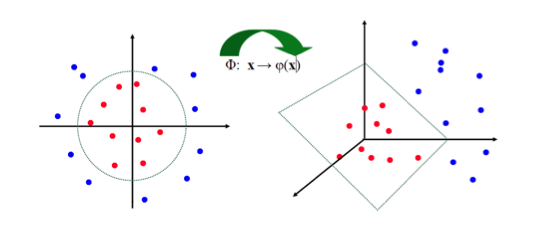
\includegraphics[width=.7\textwidth]{images/kernels.png}
\caption{ Kerneli preslikavanje }
\label{img:kernels}
\end{figure}

\noindent
Uvodi se kernel funkcija koja odgovara skalarnom proizvodu funkcija u preslikanom, novom prostoru.  Kernel funkcija se označava na sledeći način:

\begin{equation}
	K(x, y) = \langle f(x),f(y) \rangle
\end{equation}

\noindent
gde su x i y n-dimenzioni vektori, a $f$ funkcija koja slika iz n-dimenzionog prostora u m-dimenzioni prostor. Uobičajeno je da je m >> n  \cite{kernel}.

Novi problem je kako naći kernel K koji odgovara skalarnom proizvodu vektora u novom prostoru. Postoje neki uobičajeni kerneli, ali takođe postoji i način kako se konstruišu. Neki od uslova koje skalarni prozivod treba da zadovolji u vektorskom prostoru su: simetričnost, neprekidnost, pozitivna definitnost i tako dalje \cite{JelenaPHD}. Svaka funkcija koja zadovolji prethodno pomenute uslove može biti korišćena kao kernel.
\noindent
Neki od primera kernela su sledeći:

\begin{enumerate}
\item Linearni kernel

\begin{equation}
	K(x, y) = x^Ty
\end{equation}

\item Polinomijalni kernel

\begin{equation}
	K(x, y) = (x\textsuperscript{T}y + c)\textsuperscript{d}, \text{c = const}
\end{equation}
\newpage
\item Gausov kernel

\begin{equation}
	K(x, y) = exp\left( - \frac{\|x-y\|\textsuperscript{2}}{\gamma} \right)
\end{equation}

\noindent
RBF(eng. Radial Basis Function) kernel je posebna vrsta Gausovog kernela.
\end{enumerate}

\chapter{Implementacija}

Prethodno opisane metode za klasifikaciju obolelih od Alchajmerove bolesti su implementirane u okviru projekta \textit{ClassificationAlzheimer} na programskom jeziku Python, i mogu se naći na sledećoj adresi \cite{github}. Zbog prirode podataka koji su korišćeni u ovom radu, oni se neće naći u javno dostupnom repozitorijumu. Osim projekta koji sadrži kod, na repozitorijumu se nalaze i još neke datoteke bitne za izradu ovog rada i njegovih eksperimenata. Repozitorijum je organizovan u sledeće direktorijume:

\begin{enumerate}
\item \textbf{ClassificationAlzheimer}

Ovaj direktorijum sadrži programski kod.

\item \textbf{Latex}

Ovaj direktorijum sadrži sve datoteke potrebne za generisanje rada, kao i verziju u \textit{tex} i \textit{pdf} verziji.

\end{enumerate}

\noindent
Projekat je podeljen na module, od kojih svaki izvršava logički povezivu grupu zadataka:

\begin{enumerate}
\item \textbf{Glavni modul}

Glavni modul projekta koji je zadužen za odabir i pokretanje potrebnih analiza.  

\item  \textbf{Modul za podešavanja}

Služi za podešavanje i čuvanje putanja do direktorijuma sa podacima, logovima i slično, za čuvanje regularnih izraza, konstantnih izraza i slično. Ovo predstavlja unificirano mesto odakle svi ostali moduli povlače podatke.

\item \textbf{Lingvistička analiza}

Modul lingvističke analize je zadužen za čitanje datoteka koje u sebi sadrže vrste reči i računanje metrika, crtanje grafova baziranih na tim metrikama i izračunavanje stastistika, u zavisnosti šta je od opcija odabrano u glavnom modulu. Čitanje datoteka koje u sebi sadrže vrste reči uključuje za svaku datoteku, tačnije za svakog pacijenta brojanje pojedinačnih vrsta reči i izračunavanje mera koje su predstavljene u četvrtom poglavlju. Nakon toga se za svakog pacijenta kreira datoteka sa njegovim imenom koja čuva te mere. Ovaj korak čuvanja podataka je odrađen kako ne bi za svako pokretanje pograma morao da se radi isti korak čitanja tekstova, već samo kada se ti tekstovi menjanju. Naredna opcija koja može da se uključi je crtanje grafova na osnovu mera koje su zapisane u prethodnom koraku. Grafovi će zajedno za rezultatima biti prikazani u narednom poglavlju. Poslednji korak je računanje statistika od sakupljenih mera za test i trening skupove i njihovo čuvanje.

\item \textbf{Modul za iscrtavanje grafova}

Za iscrtavanje grafova je korišćena biblioteka \textit{Matplotlib}. Ona sadrži funkcije za crtanje grafova sa jednim i dva grafa na slici i za podešavanje opisa, labela, boja i slično.

\item \textbf{Modul za već poznate algoritme mašinskog učenja koristeći dokumente}

Ovaj modul je zadužen za pokretanje klasifikatora metode potpornih vektora. Prvo se čitaju podaci iz datoteka koje sadrže vrste reči i leme. Onda se formiraju trening i test skup, uz to da je x deo trening i test skupa niz tekstova, dok je y deo trening i test skupa generisan od reči "Pozitivan" i "Negativan", takvim redosledom kakvim su složeni dokumenti u x delu skupa. U okviru formiranja skupa se rade i koraci pretprocesiranja teksta, a koje vrste pretprocesiranja se rade se kontroliše promenljivima iz glavnog modula. Sledeći korak je enkodiranje y delova skupova, tako da umesto ”Pozitivan” i ”Negativan” sadrže 0 i 1, u potrebnom redosledu. Zatim se pristupa vektorizaciji reči gde se u odnosu na određeni parametar x deo skupa za trening i test predstavljaju vrećom reči ili n-gramima reči ili karaktera, a zatim se od toga kreira \textit{FA-IFD} mera.  Ovaj proces je opisan u poglavlju \ref{sec:vrt} gde se predstavljaju vektorske reprezentacije reči. Sledeći korak je pokretanje \textit{svm klasifikatora}.    
\newpage
\noindent
Korišćen je svm klasifikator sa linearnim kernelom. Klasifikator se kreira, a zatim se trenira na trening skupu, pa se vrši predikcija i određuje tačnost modela. Za implemetaciju je korišćena \textit{Sklearn} biblioteka.


\item \textbf{Modul za već poznate algoritme mašinskog učenja koristeći lingvističke mere}

I ovaj modul kao prethodni se bavi pokretanjem klasifikatora metode potpornih vektora,  ali sa drugačijim ulazom.  U prethodnom su se   koristili transformisani zapisi intervjua,  dok u ovom ulazi predstavljaju vektori vrednosti koje su sakupljene tokom lingvističke analize.  X deo trening i test skupa je niz nizova ovih promenljivih,  gde svaki niz sadrži vrednosti za po jednu osobu.  Y deo test i trening skupa je generisan od reči "Pozitivan" i "Negativan", takvim redosledom kakvim su složeni dokumenti u x delu skupa.  Prvi korak je sakupljanje statistika za svaki dokument i slaganje u niz. Pretprocesiranje u ovom slučaju nije potrebno. Sledeći korak je enkodiranje y delova skupova, tako da umesto "Pozitivan" i "Negativan" sadrže 0 i 1, u potrebnom redosledu.  Nakon toga se kreira klasifikator i trenira sa podacima iz x i y delovima trening skupa, zatim se vrši predikcija na test skupu, pa evaluacija modela. Za implementaciju je korišćena, kao i u prethodnom slučaju, \textit{Sklearn} biblioteka. 

\end{enumerate}

\chapter{Rezultati}

U prethodnim poglavljima su prikazane metode korišćene za rešavanje zadatka klasifikacije obolelih od Alchajmerove bolesti kao i detalji implementacije.  Klasifikacija je vršena metodama lingvističke analize, a zatim i koristeći već poznate metode mašinskog učenja, pa će tako rezultati i biti podeljeni.  U narednim sekcijama će biti prikazani rezultati dobijeni eksperimentima na realnim podacima. 

Da bi se izračunale mere, bilo je neophodno tekst dobijen zapisivanjem razgovora sa obolelima prvo obraditi. Potrebno je bilo ispravno razdvojiti rečenice, obratiti pažnju na pravopis i na greške u zapisivanju, kao i iz transkripata izuzeti bilo koju reč koja nije izgovorena od strane obolelog. Zatim su sklonjene oznake za pauze koje su bile zapisane u vidu "$\_$" za svaku sekundu u toku pauze u izgovoru rečenice.  Izuzeta su i pitanja osobe koja je intervjuisala, kao i oznake da oboleli govori, tačnije njegovo ime zapisano unutar "$\{\}$".  Korpus podataka se sastoji iz 23 intervjua sa obolelim koje nazivamo \textit{pozitivnim skupom} i označavamo ga sa \textit{P},  kao i 57 intervjua sa starijim nedementnim licima koje nazivamo \textit{negativnim skupom} i označavamo sa \textit{N}. 
Tekst je zatim obrađen tako da je za svaku reč određena njena vrsta reči u rečenici.  Korišćena su tri različita alata, ali zbog obima će biti prikazani samo rezultati dobijeni korišćenjem jednog.  Nije primećena značajna razlika prilikom poređenja rezultata metrika koje su izračunate pomoću izlaza iz različitih algoritama.  
\newpage
\section{Rezultati lingvističke analize}

Metode klasifikacije na osnovu lingvističke analize teksta su predstavljene u poglavlju četiri.  Mere koje su korišćene su odabrane na osnovu rezultata iz prethodnih studija vezanih za procesiranje prirodnog jezika specifično na problemu klasifikacije obolelih od Alchajmerove bolesti. Neke od mera su izabrane i kao eksperimentalne, kako bi se ispitalo da li postoji još neki način za bolju klasifikaciju.  Prikazani će biti grafikoni na kojima se vide vrednosti mera na celom skupu, a zatim i proces klasifikacije i njegova evaluacija. 

\subsection{Pregled mera na celom skupu}

U nastavku će biti prikazani neki od grafikona koji pokazuju vrednosti mera na celom skupu, kao i normalizovane vrednosti mera brojem reči u dokumentu.  Korišćene mere su sledeće: broj reči u dokumentu,  prosečna dužina izgovorenih reči,  broj imenica izgovorenih, broj prideva,  broj priloga, broj veznika,  broj zamenica,  broj veznika,  broj glagola,  odnos broja imenica i glagola, odnos broja zamenica i imenica,  Odnos tipa tokena, Bruneov indeks kao i Onoreova statistika. 

\subsubsection{Broj reči u dokumentu i prosečna dužina izgovorenih reči}

\begin{figure}[h!]
\centering
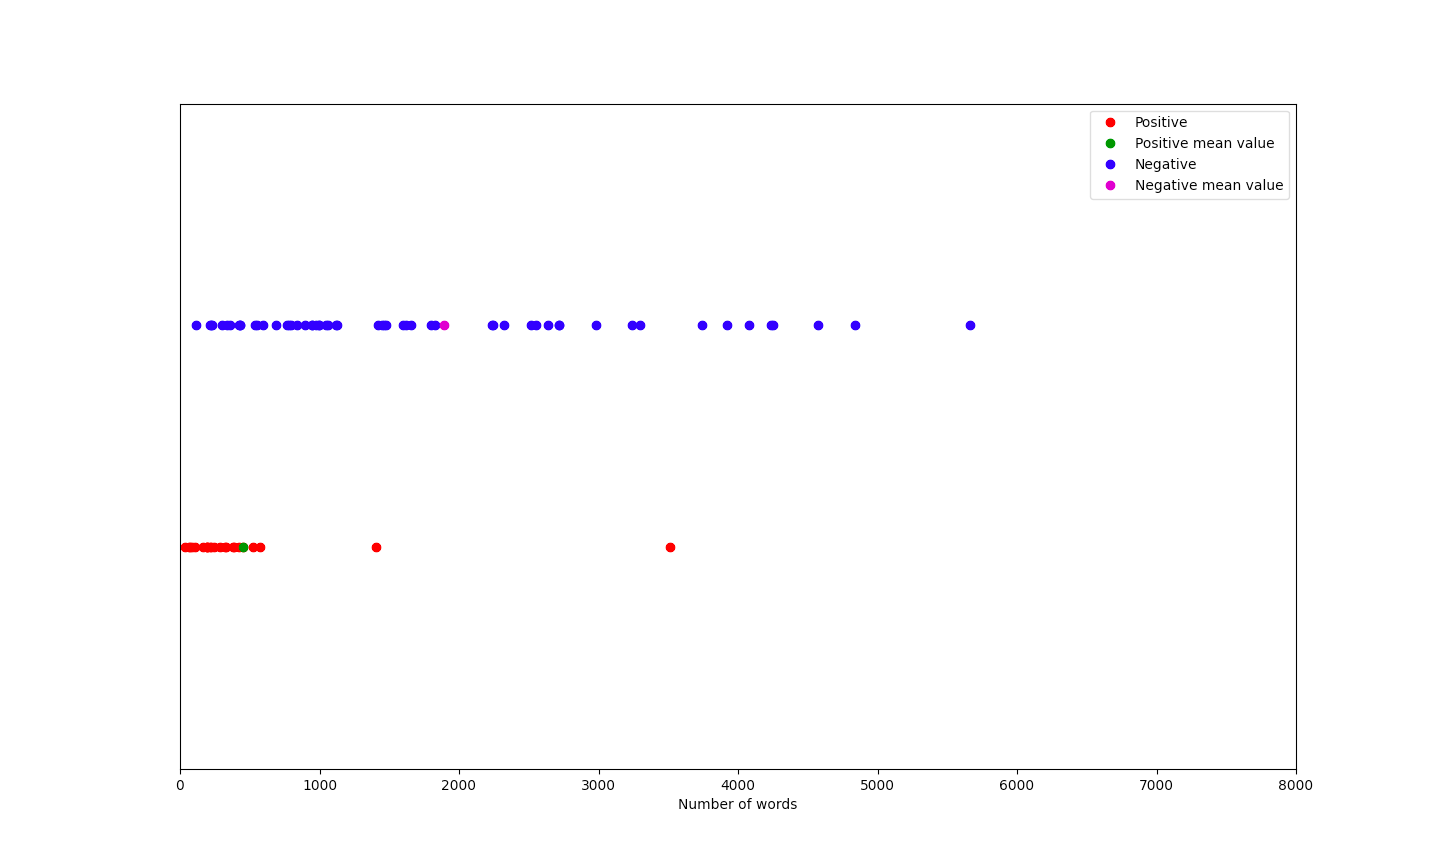
\includegraphics[width=.9\textwidth]{images/reci.png}
\caption{ Broj reči u dokumentu }
\label{img:brojreci}
\end{figure}

\begin{figure}[h!]
\centering
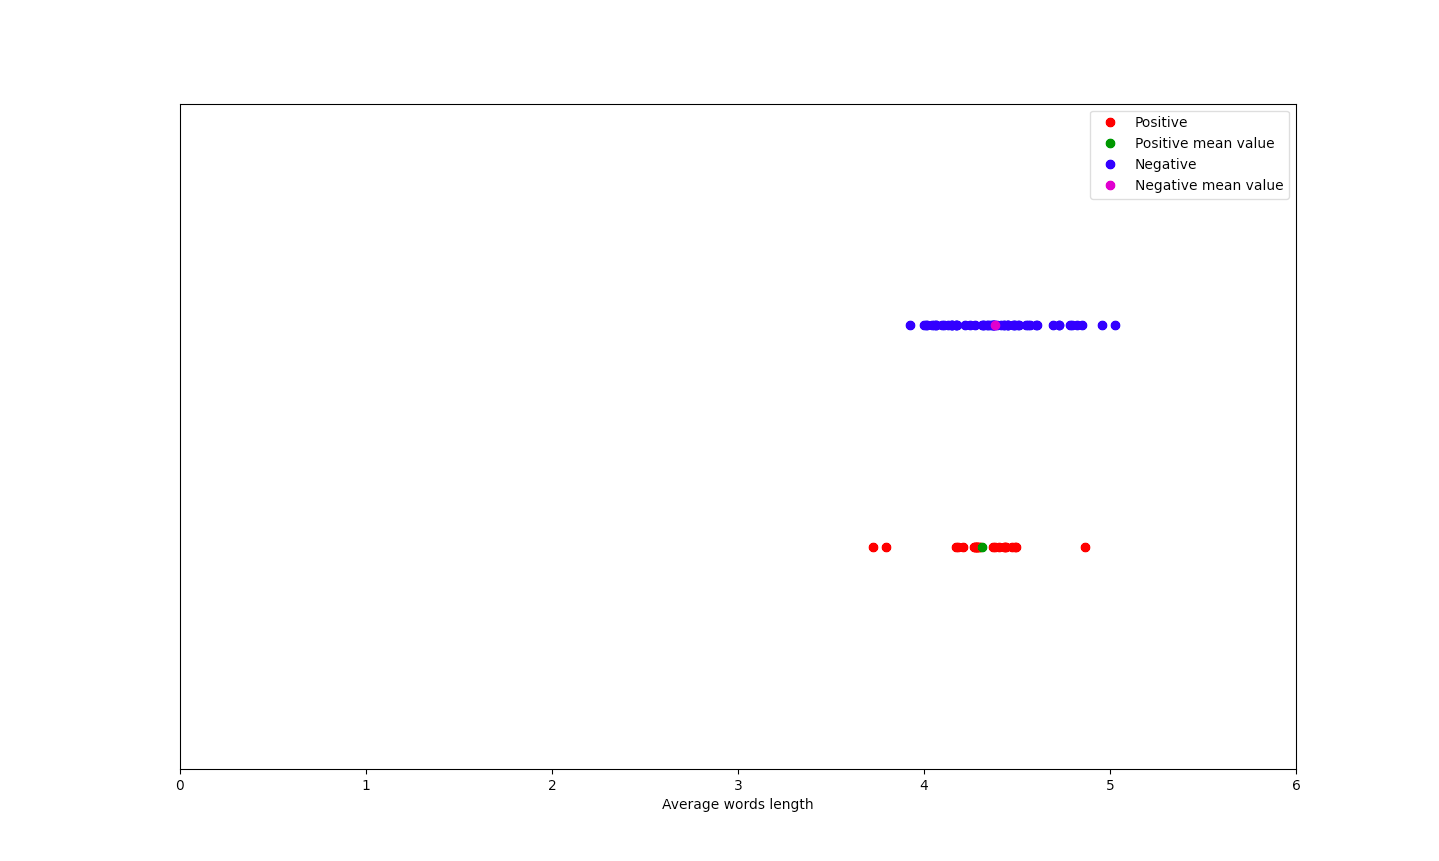
\includegraphics[width=.9\textwidth]{images/duzinareci.png}
\caption{ Prosečna dužina izgovorenih reči }
\label{img:duzinareci}
\end{figure}

Iz grafika \ref{img:brojreci} se vidi da je dužina teksta u skupu negativnih nešto veća, ali to zavisi od samog načina prikupljanja podataka.  Prosećna dužina reči je približna u oba skupa i to se vidi na grafiku \ref{img:duzinareci}.

\FloatBarrier

\subsubsection{Odnos tipa tokena}

Na grafiku \ref{img:ttr} je prikazan broj koji predstavlja vrednost mere Odnos tipa tokena (eng. Type Token Ratio). Odnos tipa tokena je mera osetljiva na dužinu teksta. Na grafikonu \ref{img:brojreci} se vidi da dokumenti u skupu pozitivnih imaju u proseku manje reči u tekstu. Kako je vrednost Odnosa Tipa tokena obrnuto proporcionalna broju reči, jasno je da su vrednosti veće za dokumente iz skupa pozitivnih.

\begin{figure}[ht!]
\centering
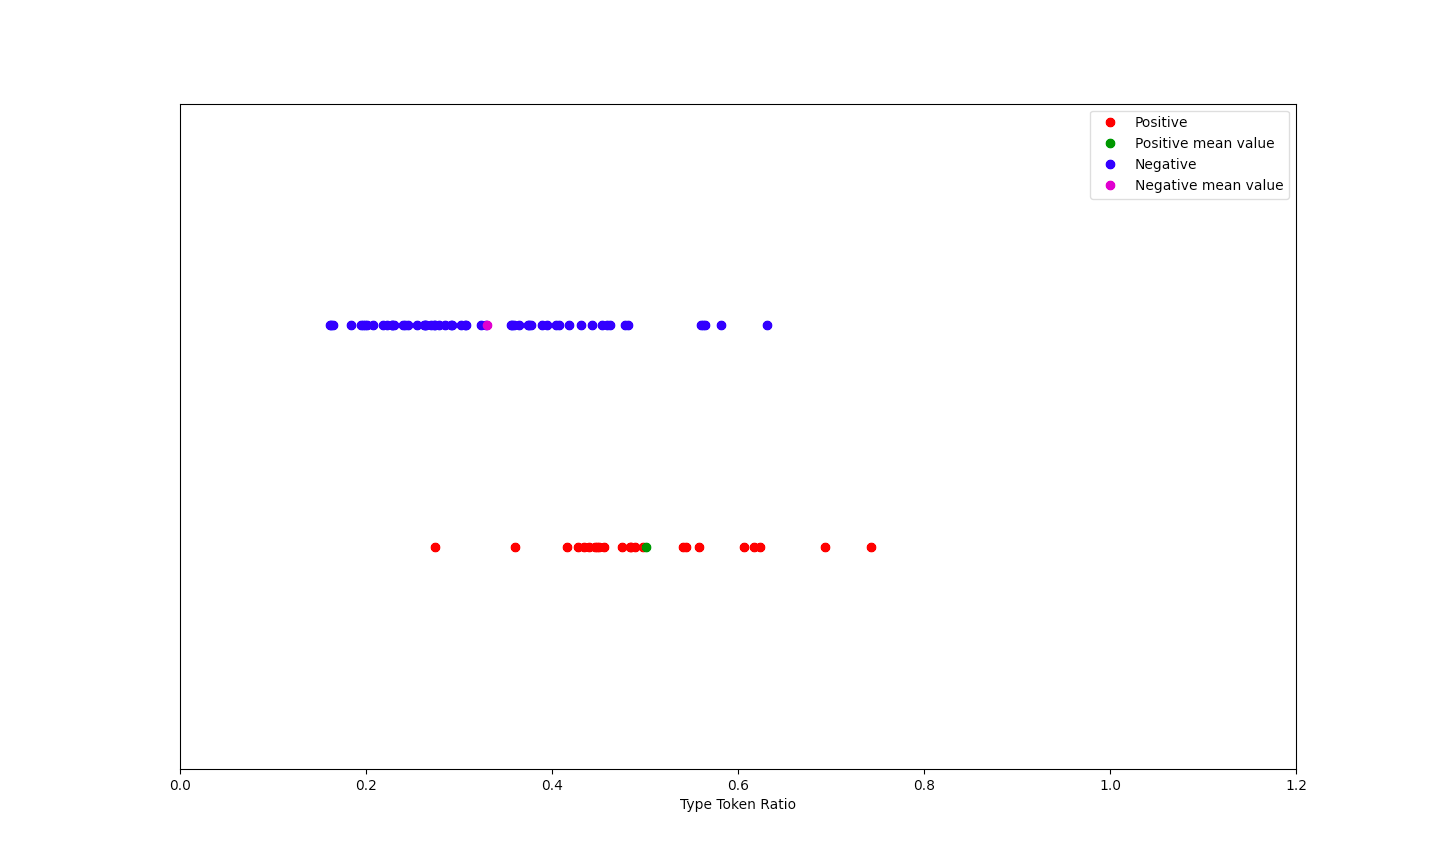
\includegraphics[width=.9\textwidth]{images/ttr.png}
\caption{ Odnos tipa tokena }
\label{img:ttr}
\end{figure}

\FloatBarrier

\subsubsection{Bruneov indeks}

Na grafiku \ref{img:r} je prikazan broj koji predstavlja vrednost mere Bruneov indeks (eng. Brunet's Index).  Bruneov indeks za dokumente u oba skupa je približno isti.  

\begin{figure}[ht!]
\centering
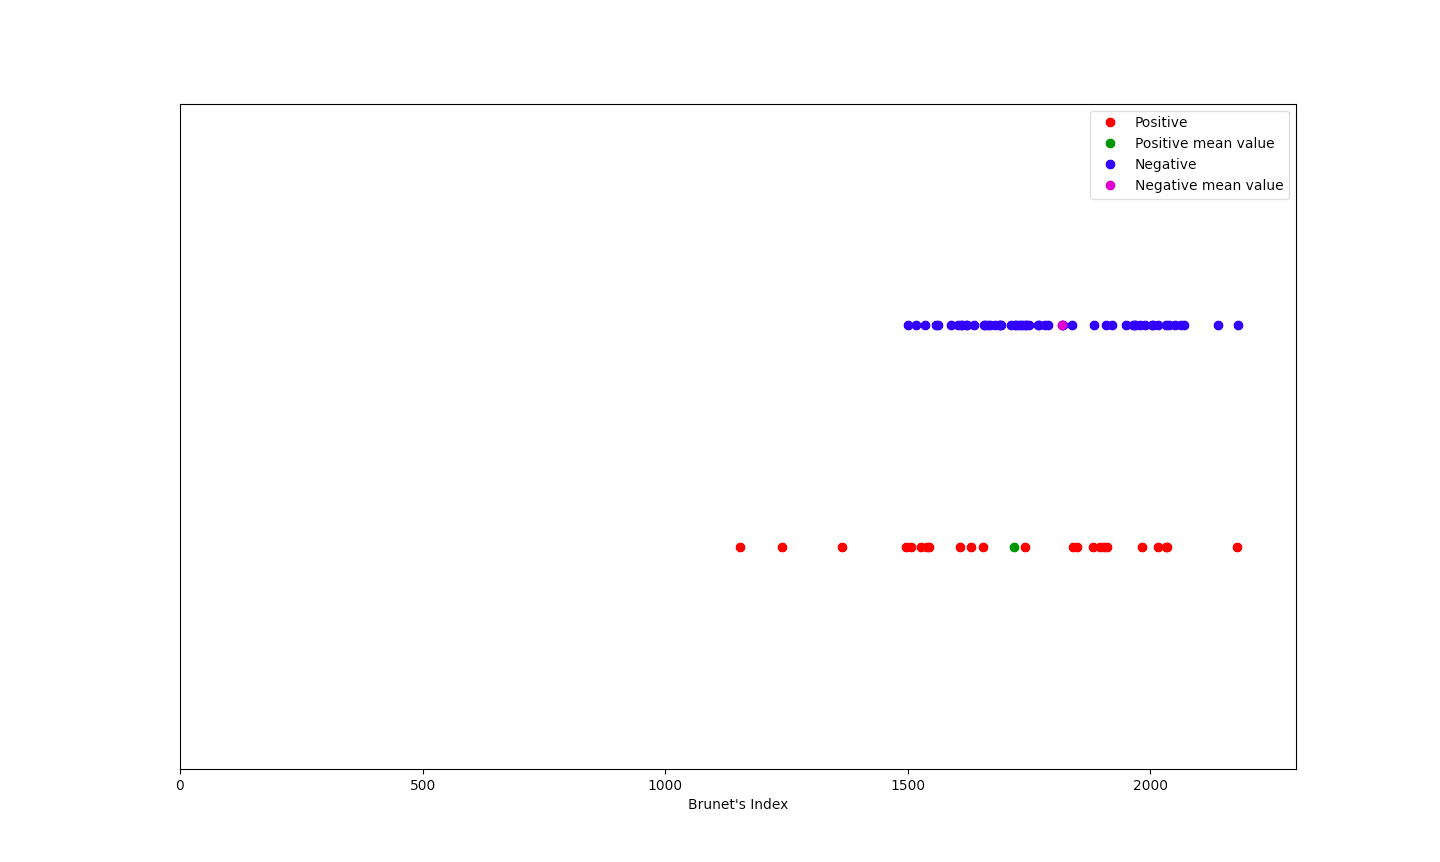
\includegraphics[width=.9\textwidth]{images/r.png}
\caption{ Bruneov indeks }
\label{img:r}
\end{figure}

\FloatBarrier

\subsubsection{Onoreova statistika}

Na grafiku \ref{img:w} je prikazan broj koji predstavlja vrednost mere Onoreova statistika (eng.  Honore's Statistic).  Vidi se da su vrednosti veće za dokumente iz skupa negativnih.

\begin{figure}[ht!]
\centering
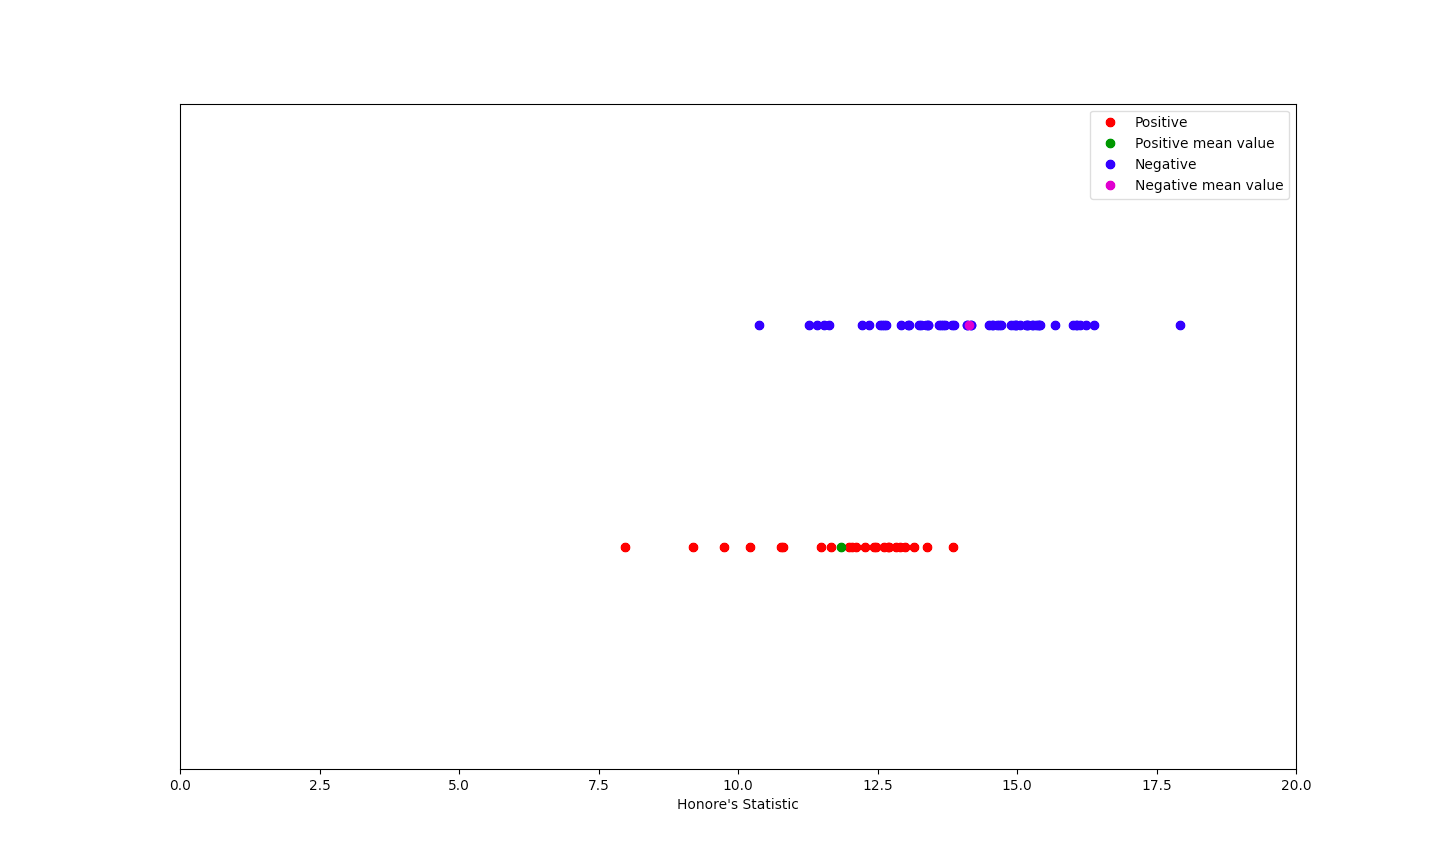
\includegraphics[width=.9\textwidth]{images/w.png}
\caption{ Onoreova statistika }
\label{img:w}
\end{figure}

\FloatBarrier

\subsubsection{Broj imenica}

Na grafiku \ref{img:imenice} je prikazan broj imenica koji je izgovoren u tekstu kao i taj broj normalizovan brojem reči u dokumentu.  Broj imenica izgovoren u odnosu na broj reči u dokumentu je nešto veći u pozitivnom skupu.  

\begin{figure}[h!]
\centering
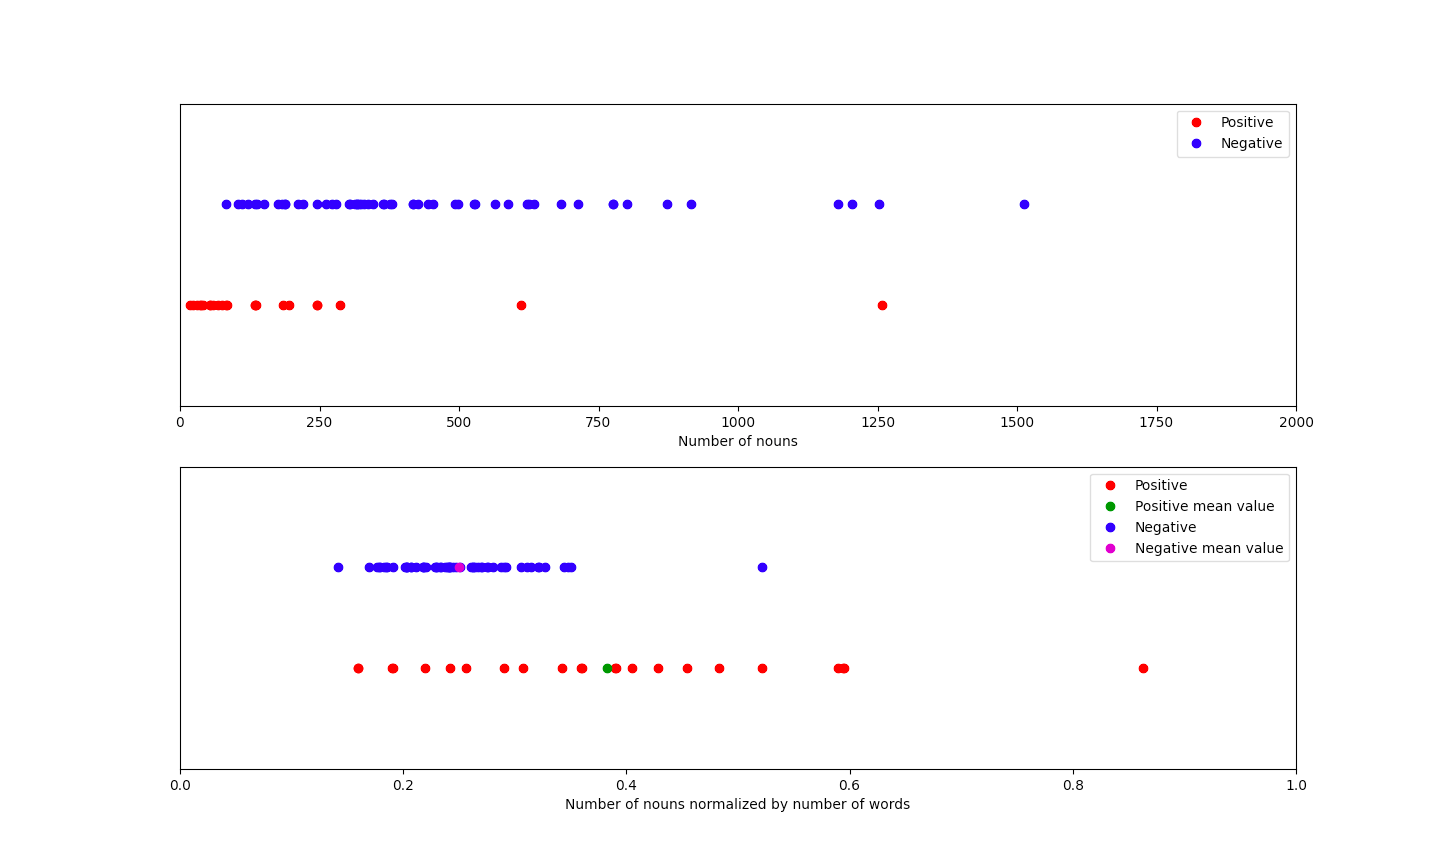
\includegraphics[width=.9\textwidth]{images/imenice.png}
\caption{ Broj izgovorenih imenica  }
\label{img:imenice}
\end{figure}

\FloatBarrier

\subsubsection{Broj zamenica}

Na grafiku \ref{img:zamenice} je prikazan broj zamenica koji je izgovoren u tekstu kao i taj broj normalizovan brojem reči u dokumentu.  Broj zamenica izgovoren u oba skupa je približno isti.  

\begin{figure}[h!]
\centering
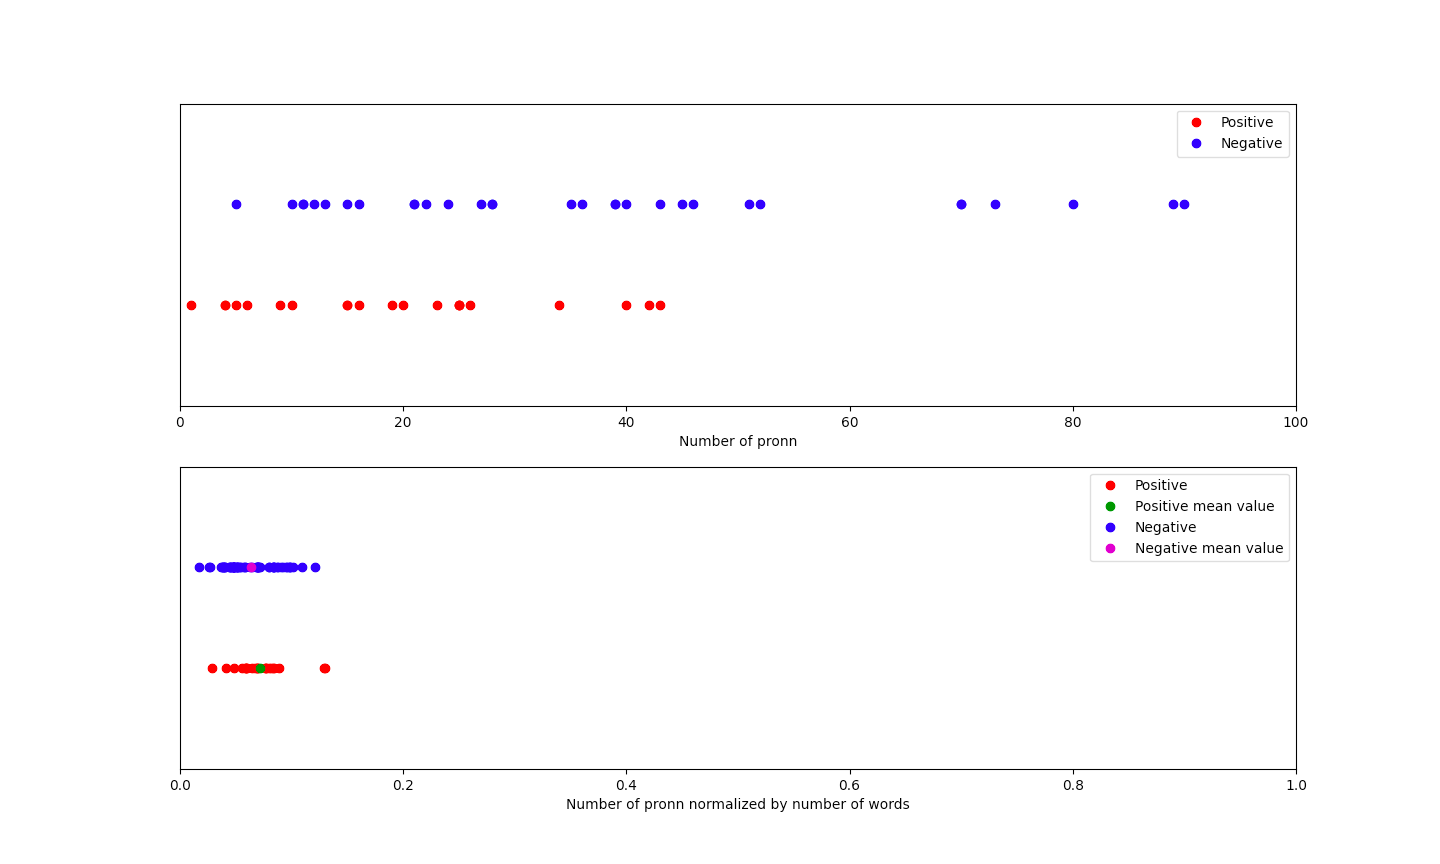
\includegraphics[width=.9\textwidth]{images/zamenice.png}
\caption{ Broj izgovorenih zamenica }
\label{img:zamenice}
\end{figure}

\FloatBarrier

\subsubsection{Broj glagola}

Na grafiku \ref{img:glagoli} je prikazan broj glagola koji je izgovoren u tekstu kao i taj broj normalizovan brojem reči u dokumentu.  Broj glagola izgovoren u oba skupa je približno isti.  

\begin{figure}[h!]
\centering
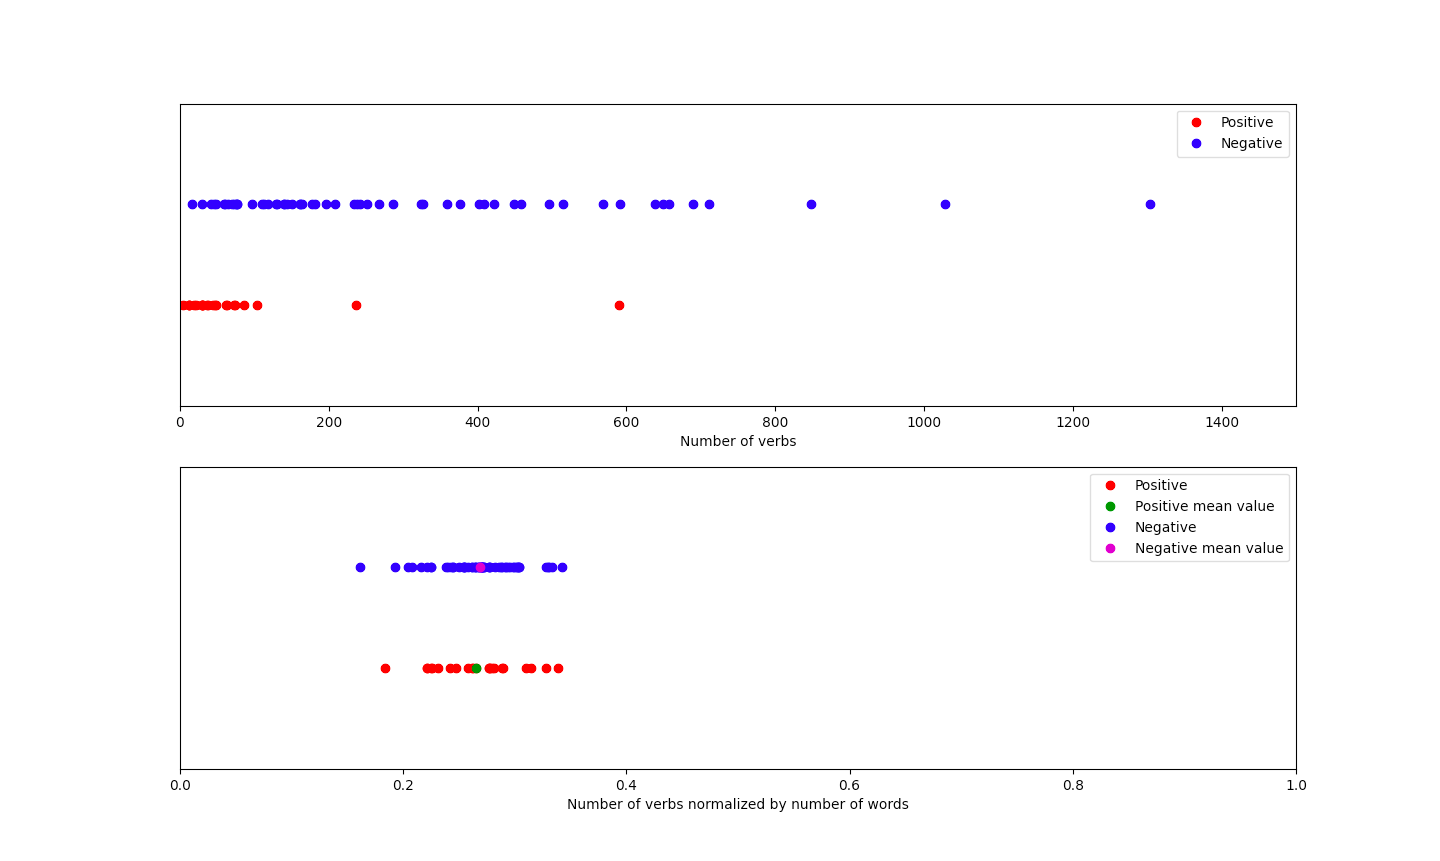
\includegraphics[width=.9\textwidth]{images/glagoli.png}
\caption{ Broj izgovorenih glagola }
\label{img:glagoli}
\end{figure}

\FloatBarrier

\subsubsection{Broj prideva}

Na grafiku \ref{img:pridevi} je prikazan broj prideva koji je izgovoren u tekstu kao i taj broj normalizovan brojem reči u dokumentu.  Broj prideva izgovoren u oba skupa je približno isti.  

\begin{figure}[ht!]
\centering
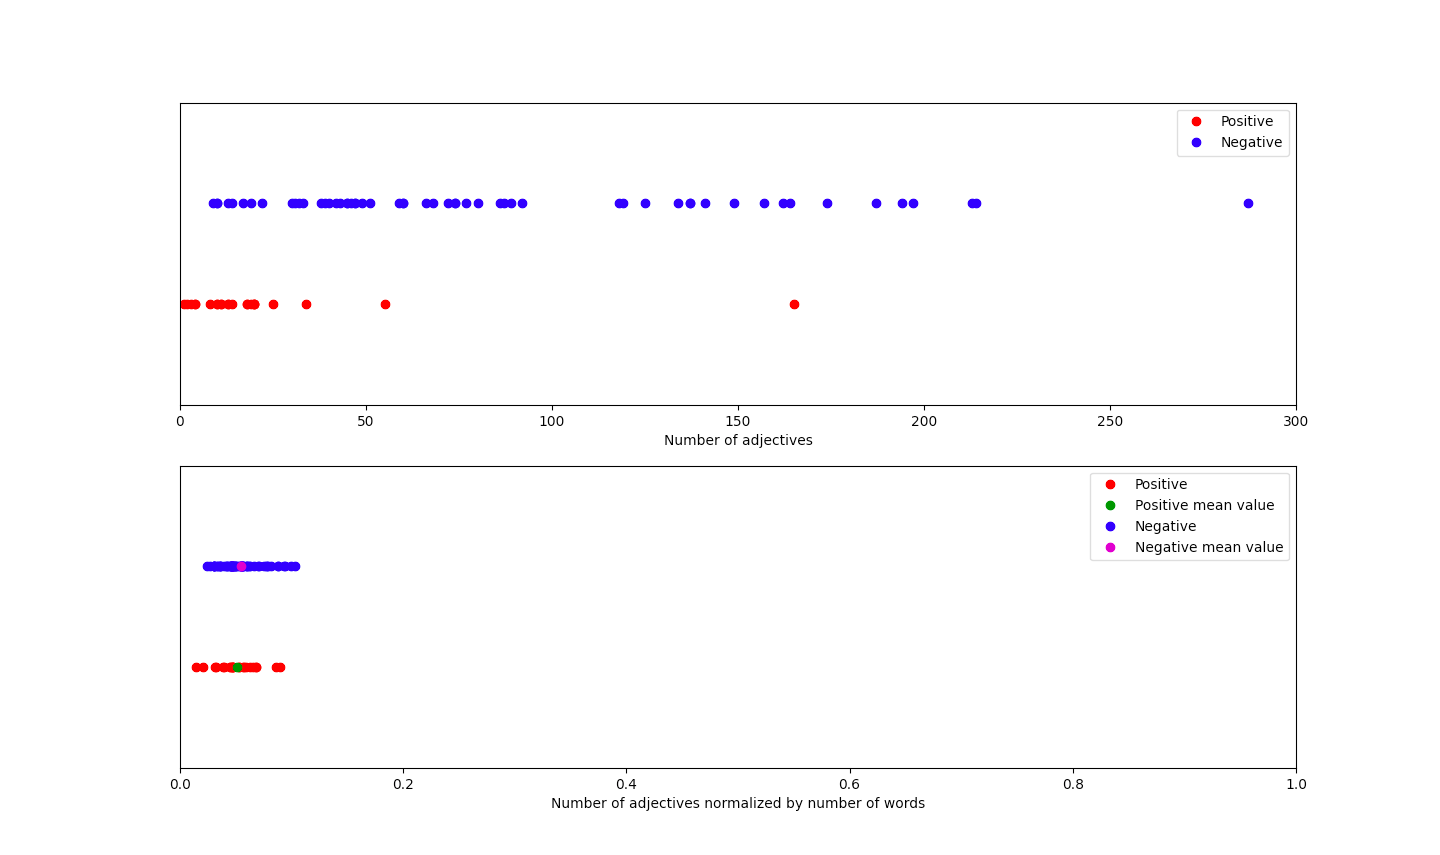
\includegraphics[width=.9\textwidth]{images/pridevi.png}
\caption{ Broj izgovorenih prideva }
\label{img:pridevi}
\end{figure}

\FloatBarrier

\subsubsection{Odnos imenica i glagola}

Na grafiku \ref{img:imenicaglagol} je prikazan broj koji predstavlja odnos broja imenica i broja glagola. 

\begin{figure}[ht!]
\centering
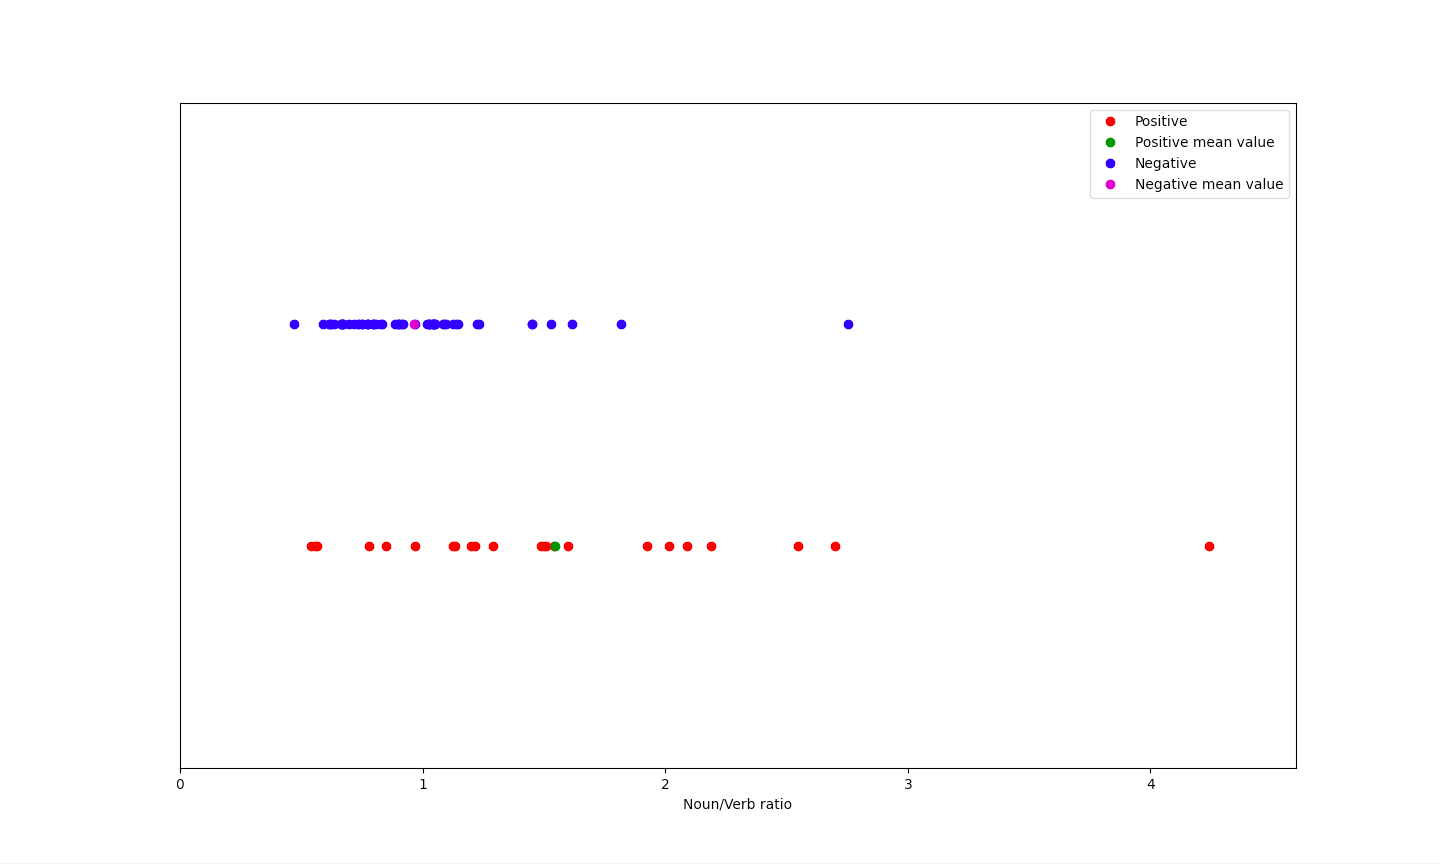
\includegraphics[width=.9\textwidth]{images/imenicaglagol.png}
\caption{ Odnos imenica i glagola }
\label{img:imenicaglagol}
\end{figure}
\newpage
\noindent
Iz prethodno prikazanih grafikona se vidi da su mere koje se najviše razlikuju na pozitivnom i negativnom skupu Odnos tipa tokena i Onoreova statistika.  Za ostale mere ne postoji tako jasna razlika kao kod pomenute dve, što će se pokazati i u evaluaciji klasifikacionog modela.
\subsection{Klasifikacija metodama leksičke analize}

Skup podataka je podeljen na šest podskupova, tako da je skup pozitivnih podeljen na tri, i negativnih na tri. U svakoj iteraciji trening skup predstavljaju dva pozitivna podskupa i dva negativna, dok test skup predstavlja jedan pozitivan i jedan negativan.  Ako podskupove označimo P\_1, P\_2 i P\_3 za pozitivan skup,  N\_1, N\_2 i N\_3 za negativan skup,  kreiran je model za sledeće trening i test skupove:

\begin{enumerate}
\item Skup 1: TRENING: P\_1, P\_2, N\_1, N\_2 TEST: P\_3, N\_3
\item Skup 2: TRENING: P\_1, P\_3, N\_1, N\_3 TEST: P\_2, N\_2
\item Skup 3: TRENING: P\_3, P\_2, N\_3, N\_2 TEST: P\_1, N\_1
\end{enumerate}

Za svaku meru je odrađena predikcija na ove tri vrste skupova i ti rezultati će biti prikazani u nastavku. Na kraju je za svaku meru određena srednja vrednost svih dobijenih vrednosti. 

\subsubsection{Odnos tipa tokena}

U nastavku su prikazane vrednosti za meru Odnos tipa tokena.  Kao što se iz rezultata vidi,  ova mera daje dobre i pouzdane rezultate na sva tri skupa.  Preciznost nije tako dobra, što nam govori da postoji određen broj instanci koje su pogrešno klasifikovane kao pozitivne, ali zato je odziv bolji,  što nam govori da nema mnogo pozitivnih instanci koje su klasifikovane kao negativne.  Ovo rezultira prilično dobrim vrednostima F-mere, što govori da postoji dobar balans u greškama napravljenim pri klasifikovanju.  Prvi model je pogrešio na 5 instanci od 26 koliko se nalazi u testnom skupu, drugi na 6 od 27, a treći na 6 od 27.   Smatra se da ova mera daje dobre rezultate pri klasifikaciji na ovim podacima, što je pokazano i u ranijim radovima koji su je razmatrali. 
\newline
\newline
\noindent\fbox{
    \parbox{\textwidth}{
	\newline
	\newline
	Stvarno pozitivni: 6 Lažno negativni: 1 \newline
	Lažno pozitivni: 4 Stvarno negativni: 15\newline
	Preciznost:0.60 Odziv: 0.86 F-mera: 0.71 \newline
	\newline
	Stvarno pozitivni: 7 Lažno negativni: 1\newline
	Lažno pozitivni: 5 Stvarno negativni: 14\newline
	Preciznost: 0.58 Odziv: 0.88 F-mera: 0.70 \newline
	\newline
	Stvarno pozitivni: 8 Lažno negativni: 0 \newline
	Lažno pozitivni: 6 Stvarno negativni: 13\newline
	Preciznost: 0.57 Odziv: 1.00 F-mera: 0.73\newline
\newline
	Prosečne vrednosti preciznosti, odziva i F-mere:\newline
	\textbf{Preciznost: 0.58 Odziv: 0.91 F-mera: 0.71}
    }
}

\subsubsection{Onoreova statistika}
U nastavku su prikazane vrednosti za meru Onoreova statistika.  Kao što se iz rezultata vidi,  i ova mera daje dobre i pouzdane rezultate na sve tri vrste skupova. Preciznost varira, što nam govori da na nekim skupovima postoji određen broj instanci koje su pogrešno klasifikovane kao pozitivne, ali zato je odziv bolji,  što nam govori da nema mnogo pozitivnih instanci koje su klasifikovane kao negativne na svim skupovima.  Prvi model je pogrešio na 5 instanci od 26 koliko se nalazi u testnom skupu, drugi na 6 od 27, a treći na 7 od 27.   Smatra se da ova mera daje dobre rezultate pri klasifikaciji na ovim podacima, što je pokazano i u ranijim radovima koji su je razmatrali.  
\newline
\newline
\noindent\fbox{
    \parbox{\textwidth}{
	\newline
	Stvarno pozitivni: 6 Lažno negativni: 1 \newline
	Lažno pozitivni: 4 Stvarno negativni: 15\newline
	Preciznost: 0.60 Odziv: 0.86 F-mera: 0.71\newline
\newline
	Stvarno pozitivni: 7 Lažno negativni: 1\newline
	Lažno pozitivni: 5 Stvarno negativni: 14\newline
	Preciznost: 0.58 Odziv: 0.88 F-mera: 0.70\newline
\newline
	Stvarno pozitivni: 7 Lažno negativni: 1 \newline
 	Lažno pozitivni: 6 Stvarno negativni: 13\newline
	Preciznost: 0.54 Odziv: 0.88 F-mera: 0.67\newline
\newline
	Prosečne vrednosti preciznosti, odziva i F-mere:\newline
	\textbf{Preciznost: 0.57 Odziv: 0.87 F-mera: 0.69}
    }
}
\newline
\newline

\subsubsection{Ostale mere}
Kod ostalih mera klasifikacija nije bila ni približno uspešna kao kod prve dve.  Prikazaćemo i takav primer koji predstavlja broj glagola.  Može se primetiti da je na svakom skupu broj pogrešno klasifikovanih instanci prilično visok, što nam pokazuje broj lažno pozitivnih i lažno negativnih. Samim tim, i F-mera za broj glagola nije dobra. 
\newline
\newline
\noindent\fbox{
    \parbox{\textwidth}{
	\newline
	Stvarno pozitivni: 2 Lažno negativni: 5 \newline
	Lažno pozitivni: 8 Stvarno negativni: 11\newline
	Preciznost: 0.20 Odziv: 0.29 F-mera: 0.24\newline
\newline
	Stvarno pozitivni: 2 Lažno negativni: 6 \newline
	Lažno pozitivni: 6 Stvarno negativni: 13\newline
	Preciznost: 0.25 Odziv: 0.25 F-mera: 0.25\newline
\newline
	Stvarno pozitivni: 7 Lažno negativni: 1 \newline
	Lažno pozitivni: 18 Stvarno negativni: 1\newline
	Preciznost: 0.28 Odziv: 0.88 F-mera: 0.42\newline
\newline
	Prosečne vrednosti preciznosti, odziva i F-mere:\newline
	\textbf{Preciznost: 0.24 Odziv: 0.47 F-mera: 0.30}
    }
}
\newline
\newline

\subsection{Zaključak klasifikacije metodama lingvističke analize}

Kod nekih mera, najveći problem pri klasifikaciji su predstavljali pozitivni dokumenti i u većini slučajeva se javljao veliki broj lažno negativnih vrednosti. Takođe,  kod nekih mera kao što je broj prideva se pojavio slučaj da ni jedan dokument nije klasifikovan kao stvarno pozitivan.  Tada nije moguće izračunati preciznost i odziv.  Takođe kod iste mere se na drugom skupu pojavio slučaj gde ni jedan dokument nije klasifikovan kao pozitivan,  ni stvarno pozitivan ni lažno pozitivan. Odatle zaključujemo da takva mera nije u stanju da razlikuje pozitivne od negativnih instanci skupova.  Od svih mera, najbolje rezultate su dali Odnos tipa tokena i Onoreova statistika. U većini ostalih mera se pojavio problem klasifikacije pozitivnih dokumenata.  

\section{Rezultati hibridnog pristupa }

Motivacija za izvođenje ove vrste eksperimenta je da se kombinuju već poznate metode mašinskog učenja sa rezultatima dobijenim primenom metoda lingvističke analize teksta u svrhu rešavanja problema klasifikacije obolelih od Alchajmerove bolesti. 
\newpage
\noindent
Svaki tekst je predstavljen atributima koji su zapravo rezultati mera dobijeni lingvističkom analizom teksta. Oni predstavljaju ulaz u metod potpornih vektora. Ovom hibridnom metodom su dobijeni sledeći rezultati:
\newline
\newline
\noindent\fbox{
    \parbox{\textwidth}{
	\newline
	Mere: Odnos tipa tokena, Bruneov indeks, Onoreova statistika \newline

	Stvarno pozitivni: 2 Lažno negativni: 6 \newline
	Lažno pozitivni: 2 Stvarno negativni: 17\newline
	Preciznost: 0.50 Odziv: 0.25 F-mera: 0.33\newline
\newline
	Stvarno pozitivni: 4 Lažno negativni: 3 \newline
	Lažno pozitivni: 1 Stvarno negativni: 18\newline
	Preciznost: 0.80 Odziv: 0.57 F-mera: 0.67\newline
\newline
	Stvarno pozitivni: 5 Lažno negativni: 3 \newline
	Lažno pozitivni: 2 Stvarno negativni: 17\newline
	Preciznost: 0.71 Odziv: 0.62 F-mera: 0.67\newline
\newline
	Prosečne vrednosti preciznosti, odziva i F-mere:\newline
	\textbf{Preciznost: 0.67 Odziv: 0.48 F-mera: 0.56}
    }
}
\newline
\newline
\noindent
Kada se za ulaze uzme niz koji sadrži Odnos tipa tokena, Bruneov indeks i Onoreovu statistiku, rezultati dobijeni su nešto lošiji na prvom skupu, ali dobri za drugi i treći.  Prosek kvari prvi skup, koji ima nisku preciznost i još niži odziv,  pa tako i lošu F-meru.
\newline
\newline
\noindent\fbox{
    \parbox{\textwidth}{
	\newline
	Mere: Odnos tipa tokena, Bruneov indeks, Onoreova statistika, broj imenica \newline

	Stvarno pozitivni: 3 Lažno negativni: 5\newline
	Lažno pozitivni: 2 Stvarno negativni: 17\newline
	Preciznost: 0.60 Odziv: 0.38 F-mera: 0.46\newline
\newline
	Stvarno pozitivni: 4 Lažno negativni: 3 \newline
	Lažno pozitivni: 2 Stvarno negativni: 17\newline
	Preciznost: 0.67 Odziv: 0.57 F-mera: 0.62\newline
\newline
	Stvarno pozitivni: 5 Lažno negativni: 3 \newline
	Lažno pozitivni: 2 Stvarno negativni: 17\newline
	Preciznost: 0.71 Odziv: 0.62 F-mera: 0.67\newline
\newline
	Prosečne vrednosti preciznosti, odziva i F-mere:\newline
	\textbf{Preciznost: 0.66 Odziv: 0.52 F-mera: 0.58}
    }
}
\newline
\newline
\noindent
Kada se u ulazni vektor doda i broj imenica normalizovan brojem reči u dokumentu,  dobijaju se bolji rezultati, pre svega na prvom skupu. Samim tim se i ukupni prosečni rezultati poboljšavaju.  Problem pravi odziv u prvom skupu, što znači da ima neki broj pozitivnih instanci koje su klasifikovane kao negativne. 
\newline
\newline
\noindent\fbox{
    \parbox{\textwidth}{
	\newline
	Mere: Odnos tipa tokena, Bruneov indeks, Onoreova statistika, broj imenica, broj glagola, broj prideva, broj priloga,  
	odnos imenica i glagola, odnos imenica i zamenica, odnos glagola i zamenica\newline

	Stvarno pozitivni: 3 Lažno negativni: 5 \newline
	Lažno pozitivni: 2 Stvarno negativni: 17\newline
	Preciznost: 0.60 Odziv: 0.38 F-mera: 0.46\newline
\newline
	Stvarno pozitivni: 3 Lažno negativni: 4 \newline
	Lažno pozitivni: 1 Stvarno negativni: 18\newline
	Preciznost: 0.75 Odziv: 0.43 F-mera: 0.55\newline
\newline
	Stvarno pozitivni: 4 Lažno negativni: 4 \newline
	Lažno pozitivni: 3 Stvarno negativni: 16\newline
	Preciznost: 0.57 Odziv: 0.50 F-mera: 0.53\newline
\newline
	Prosečne vrednosti preciznosti, odziva i F-mere:\newline
	\textbf{Preciznost: 0.64 Odziv: 0.43 F-mera: 0.51}
    }
}
\newline
\newline
Kada se u vektor dodaju sve vrednosti koje smo razmatrali u okviru lingvističke analize,  dobijamo rezultate koji su lošiji nego u prethodnom slučaju. To znači da dodavanje ostalih statistika koje su i u okviru lingvističke analize ne doprinosi boljim rezultatima.  Svi ostali modeli napravljeni na sličan način, kao ovi prikazani, su imali lošije performanse i neće biti prikazani u okviru ovog rada.  Najbolje se pokazao onaj koji sadrži Odnos tipa tokena, Bruneov indeks, Onoreovu statistiku i normalizovan broj imenica. 
\newpage
\section{Rezultati za već poznate algoritme mašinskog učenja}

U okviru ovog poglavlja biće prikazani rezultati dobijeni primenom metoda mašinskog učenja korišćenjem uobičajenih atributa: vreće reči i n-grama.  U okviru pretprocesiranja su korišćene tehnike izbacivanja stop reči,  prevođenja velikih slova u mala,  izbacivanja znakova interpunkcije kao i korišćenja lema umesto reči.  Dokumenti su predstavljeni vrećom reči i n-gramima reči i karaktera, a zatim je nad ovim reprezentacijama kreirana FA-IFD mera.  

\subsection{Vreća reči}
\noindent
Program je pokrenut za tip atributa vreća reči sa i bez pretprocesiranja.  Tekst se predstavlja identično za vreću reči kao i za unigrame. Kao algoritam mašinskog učenja korišćen je metod potpornih vektora. Rezultati su sledeći:
\newline
\newline
\noindent\fbox{
    \parbox{\textwidth}{
	\newline
	 Vreća reči, korišćenje lema=False,  izbacivanje stop reči=False,  izbacivanje znakova interpunkcije=False
\newline

	Stvarno pozitivni: 3 Lažno negativni: 5\newline
	Lažno pozitivni: 0 Stvarno negativni: 19\newline
	Preciznost: 1.00 Odziv: 0.38 F-mera: 0.55\newline
\newline
	Stvarno pozitivni: 4 Lažno negativni: 4\newline
	Lažno pozitivni: 1 Stvarno negativni: 18\newline
	Preciznost: 0.80 Odziv: 0.50 F-mera: 0.62\newline
\newline
	Stvarno pozitivni: 3 Lažno negativni: 5 \newline
	Lažno pozitivni: 0 Stvarno negativni: 19\newline
	Preciznost: 1.00 Odziv: 0.38 F-mera: 0.55\newline
\newline
	Prosečne vrednosti preciznosti, odziva i F-mere:\newline
	\textbf{Preciznost: 0.93 Odziv: 0.42 F-mera: 0.57}
    }
}
\newline
\newline
\noindent\fbox{
    \parbox{\textwidth}{
	\newline
	 Vreća reči, korišćenje lema=True,  izbacivanje stop reči=True,  izbacivanje znakova interpunkcije=True
\newline

	Stvarno pozitivni: 5 Lažno negativni: 3\newline
	Lažno pozitivni: 0 Stvarno negativni: 19\newline
	Preciznost: 1.00 Odziv: 0.62 F-mera: 0.77\newline
\newline
	Stvarno pozitivni: 4 Lažno negativni: 4 \newline
	Lažno pozitivni: 0 Stvarno negativni: 19\newline
	Preciznost: 1.00 Odziv: 0.50 F-mera: 0.67 \newline
\newline
	Stvarno pozitivni: 4 Lažno negativni: 4 \newline
	Lažno pozitivni: 0 Stvarno negativni: 19\newline
	Preciznost: 1.00 Odziv: 0.50 F-mera: 0.67\newline
\newline
	Prosečne vrednosti preciznosti, odziva i F-mere:\newline
	\textbf{Preciznost: 1.00 Odziv: 0.54 F-mera: 0.70}
    }
}
\newline
\newline
\noindent
Kada se pogledaju prethodno prikazani rezultati, vidi se da je preciznost i sa i bez pretprocesiranja vrlo dobra. Nešto lošiji su rezultati odziva. Kada se uporede rezultati sa i bez pretprocesiranja, vidi se da su oni sa pretprocesiranjem bolji u segmentu odziva, pa tako i u f-meri. 
\newpage
\subsection{N-grami karaktera}
\noindent
Program je pokrenut za n=1,2,3,4,5,6,7,8,9. Rezultati sa n-gramima karaktera su sledeći:
\newline
\newline
\noindent\fbox{
    \parbox{\textwidth}{
	\newline
	 n-gram: n=2 tip:karakteri
\newline

	Stvarno pozitivni: 1 Lažno negativni: 7 \newline
	Lažno pozitivni: 0 Stvarno negativni: 19\newline
	Preciznost: 1.00 Odziv: 0.12 F-mera: 0.22\newline
\newline
	Stvarno pozitivni: 3 Lažno negativni: 5 \newline
	Lažno pozitivni: 0 Stvarno negativni: 19\newline
	Preciznost: 1.00 Odziv: 0.38 F-mera: 0.55\newline
\newline
	Stvarno pozitivni: 3 Lažno negativni: 5 \newline
	Lažno pozitivni: 0 Stvarno negativni: 19\newline
	Preciznost: 1.00 Odziv: 0.38 F-mera: 0.55\newline
\newline
	Prosečne vrednosti preciznosti, odziva i F-mere:\newline
	\textbf{Preciznost: 1.00 Odziv: 0.29 F-mera: 0.44}
    }
}
\newline
\newline
\noindent
Za n-grame karaktera gde je n=2 se može videti da se dostiže preciznost 1. Vrednost odziva je nešto manja, iz čega se zaključuje da postoji veći broj pozitivih instanci koje su klasifikovane kao negativne. F-mera ne daje najbolje rezultate, upravo zbog slabog odziva. 
\newline
\newline
\noindent\fbox{
    \parbox{\textwidth}{
	\newline
	 n-gram: n=3 tip:karakteri
\newline

	Stvarno pozitivni: 4 Lažno negativni: 4 \newline
	Lažno pozitivni: 0 Stvarno negativni: 19\newline
	Preciznost: 1.00 Odziv: 0.50 F-mera: 0.67\newline
\newline
	Stvarno pozitivni: 5 Lažno negativni: 3 \newline
	Lažno pozitivni: 0 Stvarno negativni: 19\newline
	Preciznost: 1.00 Odziv: 0.62 F-mera: 0.77\newline
\newline
	Stvarno pozitivni: 6 Lažno negativni: 2 \newline
	Lažno pozitivni: 0 Stvarno negativni: 19\newline
	Preciznost: 1.00 Odziv: 0.75 F-mera: 0.86\newline
\newline
	Prosečne vrednosti preciznosti, odziva i F-mere:\newline
	\textbf{Preciznost: 1.00 Odziv: 0.62 F-mera: 0.76}
    }
}
\newline
\newline
\noindent
Za n-grame karaktera gde je n=3 se može videti da se dostiže preciznost 1. Odziv je dobar, što se zaključuje iz toga što je mali broj pozitivih instanci koje su klasifikovane kao negativne. Kada su preciznost i odziv dobri, očekivana je dobra F-mera koja se može videti u rezultatima.
\newline
\newline
\noindent\fbox{
    \parbox{\textwidth}{
	\newline
	 n-gram: n=4 tip:karakteri
\newline
	Stvarno pozitivni: 6 Lažno negativni: 2 \newline
	Lažno pozitivni: 0 Stvarno negativni: 19\newline
	Preciznost: 1.00 Odziv: 0.75 F-mera: 0.86\newline
\newline
	Stvarno pozitivni: 6 Lažno negativni: 2\newline
	Lažno pozitivni: 1 Stvarno negativni: 18\newline
	Preciznost: 0.86 Odziv: 0.75 F-mera: 0.80\newline
\newline
	Stvarno pozitivni: 8 Lažno negativni: 0 \newline
	Lažno pozitivni: 0 Stvarno negativni: 19\newline
	Preciznost: 1.00 Odziv: 1.00 F-mera: 1.00\newline
\newline
	Prosečne vrednosti preciznosti, odziva i F-mere:\newline
	\textbf{Preciznost: 0.95 Odziv: 0.83 F-mera: 0.89}
    }
}
\newline
\newline
\noindent
Rezultati za n-grame karaktera gde je n=4 su među najboljima, kao što je i očekivano zbog rezultata koja su pokazala slična istraživanja u ovoj oblasti, kao i prosečne dužine reči u srpskom jeziku. Ovde primećujemo klasifikaciju bez greške na trećem skupu, kao i jako visoke sve mere na svim skupovima. 
\newline
\newline
\noindent\fbox{
    \parbox{\textwidth}{
	\newline
	 n-gram: n=5 tip:karakteri
\newline
	Stvarno pozitivni: 5 Lažno negativni: 3 \newline
	Lažno pozitivni: 0 Stvarno negativni: 19\newline
	Preciznost: 1.00 Odziv: 0.62 F-mera: 0.77\newline
\newline
	Stvarno pozitivni: 6 Lažno negativni: 2  \newline
	Lažno pozitivni: 0 Stvarno negativni: 19\newline
	Preciznost: 1.00 Odziv: 0.75 F-mera: 0.86\newline
\newline
	Stvarno pozitivni: 8 Lažno negativni: 0 \newline
	Lažno pozitivni: 0 Stvarno negativni: 19\newline
	Preciznost: 1.00 Odziv: 1.00 F-mera: 1.00\newline
\newline
	Prosečne vrednosti preciznosti, odziva i F-mere:\newline
	\textbf{Preciznost: 1.00 Odziv: 0.79 F-mera: 0.88}
    }
}
\newline
\newline
\noindent
Rezultati za n-grame karaktera gde je n=5 su među najboljima, kao što je i očekivano zbog rezultata koja su pokazala slična istraživanja u ovoj oblasti, kao i prosečne dužine reči u srpskom jeziku.. Ovde primećujemo klasifikaciju bez greške na trećem skupu, kao i jako visoke sve mere na svim skupovima. Ovi rezultati su nešto slabiji nego za n=4 i ovo najavljuje trend pada performansi narednih modela.
\newline
\newline
\noindent\fbox{
    \parbox{\textwidth}{
	\newline
	 n-gram: n=6 tip:karakteri
\newline
	Stvarno pozitivni: 2 Lažno negativni: 6 \newline
	Lažno pozitivni: 0 Stvarno negativni: 19\newline
	Preciznost: 1.00 Odziv: 0.25 F-mera: 0.40\newline
\newline
	Stvarno pozitivni: 3 Lažno negativni: 5 \newline
	Lažno pozitivni: 0 Stvarno negativni: 19\newline
	Preciznost: 1.00 Odziv: 0.38 F-mera: 0.55\newline
\newline
	Stvarno pozitivni: 6 Lažno negativni: 2 \newline
	Lažno pozitivni: 0 Stvarno negativni: 19\newline
	Preciznost: 1.00 Odziv: 0.75 F-mera: 0.86\newline
\newline
	Prosečne vrednosti preciznosti, odziva i F-mere:\newline
	\textbf{Preciznost: 1.00 Odziv: 0.46 F-mera: 0.60}
    }
}
\newline
\newline
Za n=6 primećujemo pad u svim vrednostima. Za sve ostale n=7,8,9 rezultati su još lošiji. Pri analizi ovih rezultata, dolazi se do zaključka da je klasifikator najbolji za n-grame karaktera gde je n=3,4,5. Takođe pristojni rezultati se dobijaju kada je za atribut korišćena vreća reči, posebno kada je urađeno pretprocesiranje. 

\chapter{Zaključak}

U današnjem svetu, u svim oblastima života se teži automatizaciji procesa koji se obavljaju manuelno kako bi se ubrzali, poboljšali, bili objektivniji i doneli veću preciznost.  Alchajmerova bolest je najčešći oblik demencije, a njom je zahvaćen veliki procenat populacije. Broj obolelih se iz godine u godinu povećava, a pretpostavka stručnjaka je da će se taj rast nastaviti. Ova bolest izaziva afaziju, progresivno pogoršanje specifičnih kognitivnih funkcija.  Jedan od prvih simptoma bolesti je otežano usvajanje novih informacija, nakon čega nastupaju poteškoće sa pamćenjem, mišljenjem, govorom i ponašanjem. Jedan od metoda dijagnostikovanja se sastoji iz struktuiranih intervjua koje izvode lekari.  Ovi intervjui često ne mogu da uoče kompleksnu prirodu nedostataka koji se pojavljuju kod obolele osobe.  Takođe, mnoga područja u svetu nemaju adekvatno obučene stručnjake koji bi bili u stanju da uspostave dijagnozu.  
Postoji velika potreba za pristupom koji bi doneo poboljšanje u preciznosti i brzini dijagnostikovanja bolesti.  Automatizovan pristup bi pored objektivnosti doprineo i tome što bi se mogao pratiti tok bolesti i potencijalan nivo poboljšanja kod obolelog u toku ili nakon neke terapije ili leka.  Do danas nije pronađen lek za ovu bolest, ali postoje neki koji olakšavaju simptome i usporavaju njen razvoj.  Upravo u tome leži motiv za ranom dijagnozom, kako bi osoba što pre dobila adekvatnu negu.  
U ovakvim istraživanjima je bitno naglasiti veliki značaj podataka, njihovog kvaliteta i količine. Specifično za ovaj problem, do podataka je jako teško doći, pa je samim tim i njihova važnost veća. Zahvaljujući pojedincima i grupi volontera sa Biološkog fakulteta u Beogradu, ali i intervjuisanim osobama koje su pristale da izdvoje vreme i budu intervjuisane, dobijen je skup podataka neprocenjive vrednosti i oni će biti korišeni u ovom radu. 
\newpage
\noindent
Ono što pojedinac izgovara je nepresušan izvor informacija o njemu i zato upravo analizom spontanog govora možemo doći do izuzetnih rezultata.  Podatke čine transkripti intervjua sa obolelim osobama i starijim nedementnim pojedincima. 
Motivacija za ovaj master rad je davanje doprinosa kreiranju automatizovane i objektivne metode dijagnostikovanja Alchajmerove bolesti i mogućnost odlučivanja da li pojedinac pripada grupi obolelih ili zdravih starijih pojedinaca.  Prate se dva pravca istraživanja, jedan lingvističkim analizama i drugi već poznatim metodama mašinskog učenja.  Pored ove dve, prikazana je i hibridna metoda koja kombinuje metode mašinskog učenja sa rezultatima dobijenim primenom metoda lingvističke analize teksta. 
Lingvističkim analizama su dobijeni najbolji rezultati za mere Odnos tipa tokena i za Onoreovu statistiku.  Rezultati već poznatim metodama mašinskog učenja pokazuju su najbolji u slučaju kada je tekst reprezentovan vrećom reči sa pretprocesiranjem i n-gramima karaktera kada je n=5. Nešto lošiji rezultati se dobijaju primenom hibridne metode, a najbolji od njih su oni dobijeni kada su kao atributi izabrani Odnos tipa tokena, Bruneov indeks, Onoreova statistika i broj imenica.  Najbolji od ovih predstavljenih rezultata iz pojedinačnih kategorija daju već poznate metode mašinskog učenja kada je tekst predstavljen n-gramima karaktera kada je n=5.  U svim izvedenim eksperimentima je primećeno da je vrednost za preciznost u većini slučajeva dobra, dok vrednost odziva varira, što se može objasniti stepenom oboljenja ispitanika, zato sto se neki oboleli svrstavaju u zdrave osobe. 
Motivacija za razvoj i poboljšavanje metoda koje bi pomogle u dijanostikovanju i određivanju stepena ove bolesti je to što je to od neprocenjivog značaja kako za obolele, tako i za njihove porodice i ljude koji ih vole.  Kako je jasno da se sve više ljudi suočava sa ovom bolešću, kao i da će se taj broj u budućnosti povećavati, teži se tome da se napravi napredak u svim sferama koje okružuju dijagnostikovanje i lečenje. 
Doprinos ovog rada se ogleda u pronalasku i prikazivanju validnih metoda za klasifikaciju obolelih na specifičnom skupu podataka, koji nikada ranije nije korišćen u ovom tipu istraživanja.  
U budućnosti se treba fokusirati na poboljšanje ovih metoda i njihove preciznosti, korišćenjem drugih algoritama ali i unapređenjem postojećih, kao i daljom analizom podataka, prilagođavanjem metoda podacima i proširenjem korpusa. 



% ------------------------------------------------------------------------------
% ------------------------------------------------------------------------------

% ------------------------------------------------------------------------------

% ------------------------------------------------------------------------------
% 
% ------------------------------------------------------------------------------
%\literatura

\bibliographystyle{amsplain}
\bibliography{Master_rad}


% ==============================================================================
% Završni deo teze i prilozi
\backmatter
% ==============================================================================


% ------------------------------------------------------------------------------
% Biografija kandidata
\begin{biografija}
  \textbf{Ljubica Peleksić} je rođena 18. novembra 1993. godine u Beogradu.  Završila je OŠ "Ivo Andrić" kao nosilac diplome "Vuk Karadžić" i Četvrtu gimnaziju u Beogradu na prirodno-matematičkom smeru odličnim uspehom.  2012. godine je upisala Matematički fakultet u Beogradu na smeru "Informatika" i završila 2015. godine.  Iste godine je upisala master studije na istom smeru.  Tokom master studija počinje da radi u firmi "RT-RK" gde radi i danas.  Bavi se kreiranjem,  pisanjem i testiranjem aplikacija na automobilskim sistemima kao i pisanjem i testiranjem softvera na istim sistemima.  
\end{biografija}
% ------------------------------------------------------------------------------


\end{document}